\documentclass[11pt]{article}

% "final" = non-anonymous camera-ready layout (course report).
\usepackage[final]{acl}

\usepackage{times}
\usepackage{latexsym}
\usepackage[T1]{fontenc}
\usepackage[utf8]{inputenc}
\usepackage{microtype}
\usepackage{inconsolata}
\usepackage{graphicx}
\usepackage{booktabs}
\usepackage{array}
\newcolumntype{P}[1]{>{\raggedright\arraybackslash}p{#1}}
\usepackage{multirow}
\usepackage{amsmath}
\usepackage{amssymb}
\usepackage{amsthm}
\usepackage{bm}
\usepackage{xcolor}
\usepackage{tikz}
\usetikzlibrary{positioning,arrows.meta,fit,calc}
\usepackage{algorithm}
\usepackage{algpseudocode}
\usepackage{enumitem}
\usepackage{url}

% ---------------------------------------------------------------------------
% Draft switches. Set \drafttrue while the paper is being filled in:
%   \pending{...}  an analysis result that a background analysis is producing (orange)
%   \expfill{...}  an experiment slot that the experiments pass fills in (blue)
%   \expnum{...}   a number taken from our internal reports, to be re-checked (blue, inline)
%   \note{...}     a note to the authors (red)
% With \draftfalse, \expnum prints its number plainly and the other three print nothing.
% ---------------------------------------------------------------------------
\newif\ifdraft
\drafttrue
\ifdraft
  \newcommand{\pending}[1]{{\color{orange!85!black}[\textbf{Analysis pending:} #1]}}
  \newcommand{\expfill}[1]{{\color{blue!70!black}[\textbf{Experiments:} #1]}}
  \newcommand{\expnum}[1]{{\color{blue!70!black}#1}}
  \newcommand{\note}[1]{{\color{red!75!black}[#1]}}
\else
  \newcommand{\pending}[1]{}
  \newcommand{\expfill}[1]{}
  \newcommand{\expnum}[1]{#1}
  \newcommand{\note}[1]{}
\fi

% ---------------------------------------------------------------------------
% Names and notation
% ---------------------------------------------------------------------------
\newcommand{\ember}{EMBER}
\newcommand{\cinder}{CINDER}
\newcommand{\cinderz}{CINDER-z}
\newcommand{\cs}{CS}
\newcommand{\gs}{GS}
\newcommand{\twj}{TWJ}
\newcommand{\R}{\mathbb{R}}
\newcommand{\vs}{\mathcal{V}^*}
\newcommand{\Sc}{\mathcal{S}_C}
\newcommand{\Sn}{\mathcal{S}_N}
\newcommand{\Fc}{\mathcal{F}_C}
\newcommand{\e}{\mathbf{e}}
\newcommand{\z}{\mathbf{z}}
\newcommand{\cvec}{\mathbf{c}}
\newcommand{\hmean}{\operatorname{HM}}
\newcommand{\Hthree}{H_{3}}

\theoremstyle{plain}
\newtheorem{proposition}{Proposition}
\theoremstyle{remark}
\newtheorem*{remark}{Remark}

\definecolor{embergrey}{HTML}{7F7F7F}
\definecolor{cinderorange}{HTML}{D55E00}
\definecolor{cinderamber}{HTML}{E69F00}
\definecolor{csblue}{HTML}{0072B2}

\title{From EMBER to CINDER:\\ Sharpen the Concept, Burn It Once in Eight Languages, Spare the Word}

\author{Semyon Guretskiy \\
  Tel Aviv University \\
  \texttt{semyong@mail.tau.ac.il} \\\And
  Ori Petel \\
  Tel Aviv University \\
  \texttt{oripetel@mail.tau.ac.il} \\\And
  Mary Arav \\
  Tel Aviv University \\
  \texttt{maryarav@mail.tau.ac.il} \\}

\begin{document}
\maketitle

\begin{abstract}
Embedding-level concept erasure removes a concept from a language model by editing its token embeddings, but it can only remove the concept features it finds.
We show that \ember{} often misses them: concept tokens are rare, and rare tokens share a common direction that groups the concept with unrelated words.
We introduce \cinder{} (Contrastive INformed Directional Embedding Removal), which sharpens the embeddings toward the concept against ordinary text, lets each feature take as many tokens as the data supports, and verifies features against a lexicon generated once per concept.
The same sharpening extends embedding-level erasure, so far limited to English, to eight languages: a single fit with the uncentred \cinderz{} edit comes within 0.02 of per-language \ember{} at an eighth of the judge calls.
We further show that the standard evaluation rewards edits that destroy the edited words, and propose a collateral-aware evaluation that charges for this damage.
Under it, \cinder{} erases concepts that \ember{} misses and, at moderate edit size, removes more, and embedding erasure is revealed to block access to a concept through its words rather than remove it from the weights.
\end{abstract}

%=====================================================================
\section{Introduction}
\label{sec:intro}
%=====================================================================

As language models (LMs) are deployed in more applications, the ability to erase specific knowledge from them becomes important for safety and compliance \citep{eldan2023harry,li2024wmdp}.
A prominent approach is \emph{persistent} concept erasure, which removes knowledge of a target concept by modifying the model's weights \citep{gurarieh2025precise,ashuach2026crisp}.
Recently, \citet{suslik2026ember} showed that such methods overlook a part of the model that stores knowledge: the token embeddings.
Their method, \ember{}, decomposes the embeddings of concept-related tokens into sparse features, selects the features of the target concept with an LLM judge, and subtracts them from a small set of tokens.\footnote{Our code is available at \url{https://github.com/guretskiysemyon/nlp_proj}.}
Combined with MLP-based methods, it substantially improves robustness to relearning.

\begin{figure}[t]
\centering
\begin{tikzpicture}[
  box/.style={draw, rounded corners=2pt, align=center, font=\scriptsize, text width=2.85cm,
              minimum height=0.86cm, inner sep=2pt},
  eb/.style={box, draw=embergrey, fill=embergrey!7},
  cb/.style={box, draw=cinderorange, fill=cinderorange!7, line width=0.6pt},
  sl/.style={font=\scriptsize\bfseries, align=right, text width=1.15cm, anchor=east},
  hd/.style={font=\footnotesize\bfseries},
  arr/.style={-{Stealth[length=3pt]}, semithick, draw=black!45}]
  \node[eb] (e1) at (0,0) {Sparse MF of raw embeddings;\\ 1\% of tokens per feature};
  \node[eb, below=0.22cm of e1] (e2) {$\rho > \tau$; LLM judge reads\\ a one-line summary};
  \node[eb, below=0.22cm of e2] (e3) {$\e_t - \delta\,\cvec_t$, with $\delta$\\ up to 200};
  \node[eb, below=0.22cm of e3] (e4) {efficacy, MMLU,\\ Alpaca coherence};
  \node[eb, below=0.22cm of e4] (e5) {English only; one fit\\ per language otherwise};
  \node[cb, right=0.25cm of e1] (c1) {\textbf{sharpen} toward the concept;\\ \textbf{one global} sparsity budget};
  \node[cb, right=0.25cm of e2] (c2) {judge \textbf{or} lexicon match\\ (one LLM call per concept)};
  \node[cb, right=0.25cm of e3] (c3) {same tokens; concept part\\ \textbf{relative to ordinary text}};
  \node[cb, right=0.25cm of e4] (c4) {+ \textbf{collateral}, edit size,\\ \textbf{word integrity}};
  \node[cb, right=0.25cm of e5] (c5) {\textbf{one fit for eight}\\ \textbf{languages}};
  \node[sl, left=0.12cm of e1] {Decompose};
  \node[sl, left=0.12cm of e2] {Identify};
  \node[sl, left=0.12cm of e3] {Erase};
  \node[sl, left=0.12cm of e4] {Evaluate};
  \node[sl, left=0.12cm of e5] {Languages};
  \node[hd, text=embergrey, above=0.05cm of e1] {\ember{}};
  \node[hd, text=cinderorange, above=0.05cm of c1] {\cinder{} (ours)};
  \foreach \a/\b in {e1/e2,e2/e3,c1/c2,c2/c3} \draw[arr] (\a) -- (\b);
  \draw[arr, dashed] (e3) -- (e4);
  \draw[arr, dashed] (c3) -- (c4);
\end{tikzpicture}
\caption{\ember{} erases a concept by decomposing token embeddings into sparse features, identifying the concept's features, and subtracting them from concept tokens. \cinder{} keeps this framework and changes how the concept is found, verified and edited, so that quiet concepts become the strongest direction of the matrix. One \cinder{} fit serves eight languages, where \ember{} needs a fit per language. We also extend the evaluation so that destroying the edited words no longer counts as erasing the concept.}
\label{fig:overview}
\end{figure}

However, an embedding edit can only remove what its features capture, and how reliably \ember{} finds a concept's features has not been studied.
Its authors note that embeddings may not be an effective target for some concepts, that the tokens selected for editing may include semantically unrelated ones, and that the edit only applies to English tokens \citep[Limitations]{suslik2026ember}.

In this work, we hypothesize that these limitations stem in part from the geometry in which \ember{} searches for features.
Specifically, sparse matrix factorization minimizes reconstruction error, so it spends its features on directions that many tokens share, such as magic, writing or books, while a concept such as Harry Potter is carried by a few rare tokens and explains little of the error.
We call such a concept \emph{quiet}: in \ember{}'s matrix, eleven generic features outrank the Harry Potter feature on \ember{}'s own concept score, and the feature's tail holds tokens such as Nestl\'e, Lego and Trump (Figure~\ref{fig:hp}).
Two more design choices compound the problem.
Every feature keeps the same 1\% of the tokens regardless of how broad its concept is, and the judge accepts a feature based on a one-sentence summary that often abstracts the concept away.
When no feature is accepted, nothing is erased.

To tackle this gap, we introduce \cinder{} (Contrastive INformed Directional Embedding Removal; Figure~\ref{fig:overview}), which keeps \ember{}'s localize-then-edit framework and changes how the concept is found.
\cinder{} whitens the embeddings against ordinary text and sharpens them toward the concept's page, so that what distinguishes the concept becomes the strongest direction in the matrix.
It shares one sparsity budget across all features, so that each feature takes as many tokens as the data supports, and it verifies features both bottom-up, with \ember{}'s judge, and top-down, against a concept lexicon generated once per concept.
Because the sharpened space is centred on ordinary text, \cinder{}'s edit removes only what distinguishes the concept; an uncentred variant, \cinderz{}, also removes part of the component that all tokens share, as \ember{}'s edit does.

Sharpening also makes multilingual erasure practical, which \ember{} leaves to future work \citep[Limitations]{suslik2026ember}.
Because \ember{} edits the rows of English tokens, a concept it erases in English largely survives in other languages: on Gemma, edited models retain \expnum{0.24} more of the concept's knowledge in German, Spanish, French and Russian than in English.
Running \ember{} separately in every language multiplies its cost by the number of languages, and fitting it once on multilingual text mostly fails, yielding a concept feature for only \expnum{10 of 38} concepts.
We expect the concept to be quieter still in a multilingual matrix, where language identity adds loud directions of its own.
\cinder{} whitens against a background with equal text in every language, which removes these directions, and sharpens toward the concept's pages in all languages.
A single \cinder{} fit over eight languages then erases as well as eight separate \ember{} runs, with one factorization and one judging pass instead of eight; to our knowledge, this is the first multilingual erasure at the embedding level.

We assess \cinder{} through experiments on Gemma-2-2B-it \citep{gemma2024gemma2} and, across eight languages, Llama-3.1-8B-Instruct \citep{grattafiori2024llama3}.
Notably, evaluating it exposed a blind spot in the standard protocol.
\ember{}'s tuning score prefers edits up to a hundred times longer than the embeddings they change, which destroy the edited words rather than remove the concept from them.
Because the concept questions contain the edited words, a destroyed word counts as erased knowledge, while MMLU and Alpaca coherence rarely encounter it.
We therefore extend the evaluation with \emph{collateral} questions that use the edited words in their other meanings (e.g., Prince Harry when erasing Harry Potter), one scale of edit size shared by all methods, and tests of whether the edited words survive.

Our results show that once collateral damage is charged for, every method moves from token-destroying edits to edits about as long as the token, and that embedding erasure blocks access to a concept through its words rather than removing it from the weights.
Within this regime, \cinder{} erases concepts that \ember{} misses (\expnum{14} vs.\ \expnum{3} runs in which only one of the methods edits), and its direction removes more at equal edit size (\expnum{$+0.15$} on the combined score, \expnum{10 of 11} held-out concepts), while at each method's own operating point the two tie.
Across eight languages, a single \cinder{} fit matches running \ember{} separately in each language (\expnum{0.23} vs.\ \expnum{0.25}) at one eighth of the selection cost, and finds concept features for twice as many concepts as a single multilingual \ember{} fit (\expnum{21} vs.\ \expnum{10} of 38).

Finally, we analyze how sharpening changes the embedding space.
We find that the model's first layer reads one direction, the mean of all embeddings, far more strongly than others, and that this shared direction, not the concept, explains why \ember{}'s edits are read more strongly than \cinder{}'s.
\pending{one or two sentences from the embedding-space analysis (\S\ref{sec:analysis}): the concept direction's energy rank, near-orthogonal features with meaningful angles, widths that follow the data, and the circularity control.}

To conclude, our work (1) diagnoses why embedding-level erasure misses quiet concepts, (2) introduces \cinder{}, which finds and erases them more reliably, (3) extends embedding-level erasure to many languages with a single fit, at one eighth of the selection cost of erasing each language separately, and (4) shows that the standard evaluation of embedding erasure rewards destroying tokens, and proposes a collateral-aware alternative that needs no LLM judge inside the tuning loop.
Overall, our findings suggest that where a concept is looked for matters as much as how it is removed, and that an embedding edit must be judged by what it does to the words it edits.


%=====================================================================
\section{Preliminaries and Notation}
\label{sec:prelim}
%=====================================================================

We follow the notation of \citet{suslik2026ember}: a transformer LM \citep{vaswani2017attention} has hidden dimension $d$, vocabulary $\mathcal V$ and input embedding matrix $E \in \R^{|\mathcal V| \times d}$, whose row $\e_t \in \R^d$ embeds token $t$.

\paragraph{Concept Erasure in Language Models}
Given a model $M$ and a target concept $C$ (e.g., Harry Potter), persistent concept erasure updates the parameters of $M$ so that it no longer answers questions about $C$ better than chance, while maintaining its performance on other concepts and tasks \citep{eldan2023harry,li2024wmdp,gurarieh2025precise,suslik2026ember}.
We assume target sentences $\Sc$ from $C$'s Wikipedia page and neutral sentences $\Sn$ from unrelated pages.

\paragraph{EMBER}
\ember{} follows a localize-then-edit approach with three stages.
(1)~\emph{Decomposing.}
Let $\vs$ be the token types that appear in $\Sc \cup \Sn$, $n = |\vs|$, and $A = E_{\vs}^{\top} \in \R^{d \times n}$.
\ember{} factorizes $A \approx ZY$, with a dictionary $Z \in \R^{d \times k}$ of \emph{embedding features} $\z_i$ and coefficients $Y \in \R^{k \times n}$, keeping the 1\% largest entries of each row of $Y$ and alternating least squares (Sparse MF).
(2)~\emph{Identifying.}
Tokens are labelled concept, neutral or both, by whether they appear in $\Sc$, $\Sn$ or both; with $T_C$ and $T_N$ the concept- and neutral-labelled tokens, each feature is scored by its mass ratio
\begin{equation}
  \rho_i = \frac{\sum_{t\in T_C} |Y_{i,t}|}{\sum_{t \in T_N} |Y_{i,t}|},
  \label{eq:rho}
\end{equation}
and features with $\rho_i > \tau = 2$ go to an LLM judge that first describes the feature's top tokens without seeing the concept, then decides from the description alone whether the feature is the concept, accepting at confidence $\geq 0.85$.
The accepted features form $\Fc$.
(3)~\emph{Erasing.}
Each concept token with $Y_{i,t} \neq 0$ for some $i \in \Fc$ is edited as
\begin{equation}
  \e_t' = \e_t - \delta\, \cvec_t, \qquad \cvec_t = \sum_{i \in \Fc} Y_{i,t}\, \z_i ,
  \label{eq:edit}
\end{equation}
where $\cvec_t$ is the token's \emph{concept part} and $\delta \geq 0$ the erasure strength.

\paragraph{Evaluating Erasure}
\ember{} measures efficacy (accuracy on multiple-choice questions about $C$), specificity (similar-domain questions and MMLU; \citealp{hendrycks2021mmlu}), coherence (AlpacaEval judged by an LLM; \citealp{taori2023alpaca}) and robustness to relearning \citep{deeb2024unlearning}; the harmonic mean $H$ of all but relearning, normalized by the unedited model, selects $\delta \in \{0.5, \dots, 200\}$ on validation questions.

%=====================================================================
\section{Why \ember{} Misses Quiet Concepts}
\label{sec:motivation}
%=====================================================================

\begin{figure*}[t]
  \centering
  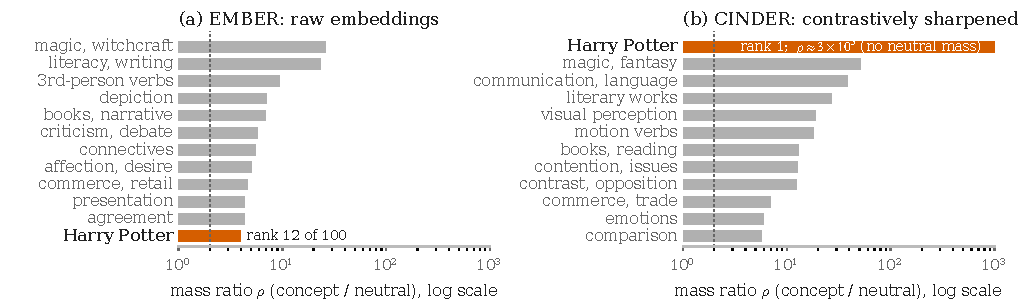
\includegraphics[width=\textwidth]{figures/hp_rho.pdf}
  \caption{Harry Potter is a quiet concept in \ember{}'s matrix and the strongest one after Contrastive Sharpening. Shown are the top 12 of 100 sparse-MF features for Harry Potter on Gemma-2-2B-it (seed 42), ranked by \ember{}'s mass ratio $\rho$ (Eq.~\ref{eq:rho}); labels paraphrase each feature's LLM description. (a)~On the raw embeddings, eleven generic topics outrank the concept feature. (b)~On the sharpened matrix, with the same 1\% row sparsity, the concept feature ranks first and has no neutral mass. The dotted line marks \ember{}'s threshold $\tau = 2$.}
  \label{fig:hp}
\end{figure*}

A natural question is how reliably \ember{}'s first two stages find the target concept.
To study this, we reproduced \ember{} on Gemma-2-2B-it, matching the published accuracies within four points (\S\ref{app:ember}), and inspected each stage on its flagship concept, Harry Potter, before testing each observation on more concepts and seeds.
We find five issues, summarized in Table~\ref{tab:diagnosis}.

\paragraph{The concept is a quiet direction}
Sparse MF minimizes the squared reconstruction error, so a feature is only as valuable to it as the energy it explains.
Intuitively, a topic shared by many tokens explains much of this energy, while a concept carried by a few dozen rare names explains little.
Figure~\ref{fig:hp}a shows the consequence for Harry Potter: eleven generic features, such as magic, writing, third-person verbs and books, score higher than the concept feature on \ember{}'s own concept ratio.
The cost appears in the feature's tail.
Its first 19 tokens all belong to Harry Potter, but only 2 of the next 11 do, and further down are Nestl\'e, Lego, Trump and Latin taxonomic suffixes, all of which \ember{} would edit (\S\ref{app:examples}).
We expect concepts to be quiet partly because their tokens are rare, and rare tokens receive fewer gradient updates during training \citep{gao2019representation}.
\pending{WP1: across 38 concepts, the energy rank of the concept direction in the raw matrix, and whether concept tokens are rarer and lower in variance.}

\paragraph{One width does not fit all concepts}
\ember{} keeps the top 1\% of tokens in every feature, 48 tokens for Harry Potter.
Since concepts differ in breadth, a fixed width cuts a broad concept short and pads a narrow one with unrelated tokens.
Ancient Rome illustrates the first case: depending on the seed, \ember{} finds it as zero, one or two features, and across 20 seeds its edited token sets overlap with a Jaccard index of only \expnum{0.26} (\S\ref{app:gs}).
\pending{WP3: across concepts, where the natural tail of the concept feature ends relative to the 1\% cut.}

\paragraph{The judge loses the concept in its summary}
\ember{}'s judge does not see the feature, only a one-sentence description of its top tokens, and the description is where concepts get lost.
In our runs, \emph{heroin} was described as ``addictive drugs'' and \emph{World War II} as ``20th-century totalitarian regimes''; both were rejected, as was Valentine's Day, each at exactly the 0.85 confidence cutoff.
A rejected concept is not erased at all, since no feature is left to subtract: on 12 held-out concepts \ember{} edits nothing in \expnum{19 of 60} runs, and a multilingual \ember{} fit finds a concept feature for only \expnum{10 of 38} concepts (\S\ref{sec:experiments}).

\paragraph{The edit stays in English}
\ember{} edits the rows of English tokens, and its authors leave other languages to future work.
We find that a concept erased in English largely survives in other languages: on Gemma, \ember{}-edited models retain \expnum{0.24} more of the concept's knowledge in German, Spanish, French and Russian than in English, and \expnum{0.41} more in Russian, whose tokens the English edit never touches (\S\ref{app:ml}).
The two obvious remedies both fall short.
Running \ember{} separately in every language multiplies the factorizations and judge calls by the number of languages, and a single \ember{} fit on multilingual text finds a concept feature for only \expnum{10 of 38} concepts on Llama-3.1-8B (\S\ref{sec:exp-ml}).
\pending{WP9: whether language identity dominates the features of the multilingual \ember{} fit.}

\paragraph{The evaluation rewards destroying tokens}
\ember{} chooses the erasure strength $\delta$ by $H$ on validation questions.
In our reproduction, this selects the largest value, $\delta = 200$, for \expnum{6 of 10} concepts.
Since the concept part $\cvec_t$ is about 0.6 of a token's length, the edited embedding is about 120 times longer than the original and points along $-\cvec_t$: the word is replaced rather than cleaned.
None of the metrics registers this.
The concept questions contain the edited words, so a destroyed word counts as erased knowledge; the similar-domain questions avoid them, the MMLU gate never binds in \expnum{344} grid points, and Alpaca coherence stays at or above \expnum{0.87}.
Free text tells a different story: at $\delta = 200$, \expnum{12 of 20} prompts that use the edited words in other senses break (asked about Prince Harry, the model describes the singer Prince), against \expnum{0--1 of 20} at $\delta = 1$.
We refer to this regime as \emph{token destruction}.

\begin{table}[t]
  \centering
  \small
  \setlength{\tabcolsep}{3pt}
  \begin{tabular}{@{}P{1.45cm}P{3.15cm}P{2.3cm}@{}}
    \toprule
    Stage & Issue & \cinder{}'s change \\
    \midrule
    Decompose & The concept is a quiet direction; its feature fills with loud neighbours & Contrastive Sharpening (\S\ref{sec:cs}) \\
    Decompose & One width for every feature & Global Sparsity (\S\ref{sec:cs}) \\
    Identify & The judge reads a summary that loses the concept & Two-Way Judge (\S\ref{sec:twj}) \\
    Erase & Centred and uncentred edits differ by a direction all tokens share & Both variants (\S\ref{sec:cinderz}) \\
    Scope & Edits English tokens only; one multilingual fit finds few concepts & One fit for eight languages (\S\ref{sec:ml}) \\
    Evaluate & Destroying a word scores as erasing a concept & Collateral-aware evaluation (\S\ref{sec:setup}) \\
    \bottomrule
  \end{tabular}
  \caption{The issues we identify in each stage of \ember{} and the change \cinder{} makes. The erasure-stage row concerns a choice in our own design rather than an issue of \ember{}.}
  \label{tab:diagnosis}
\end{table}

%=====================================================================
\section{\cinder{}}
\label{sec:method}
%=====================================================================

To find quiet concepts and erase them, we propose \cinder{}.
\cinder{} follows \ember{}'s localize-then-edit approach and changes each of its three stages: (1)~decomposing a contrastively sharpened embedding matrix under a global sparsity budget (\S\ref{sec:cs}), (2)~identifying concept-related features with a two-way judge (\S\ref{sec:twj}), and (3)~erasing them, with or without the component that all tokens share (\S\ref{sec:cinderz}).
Finally, we extend the pipeline to many languages with a single fit (\S\ref{sec:ml}).
\cinder{} keeps \ember{}'s data $\Sc$, $\Sn$ and $\vs$, its Sparse MF algorithm, its $\rho$ filter and the form of its edit (Eq.~\ref{eq:edit}).

\subsection{Finding Concept Features in a Sharpened Space}
\label{sec:cs}

Sparse MF finds the directions that explain the most energy of the matrix it is given (\S\ref{sec:motivation}).
Rather than changing the factorization, we change the matrix, so that the concept carries the energy.
Whitening is a standard step before sparse coding \citep{hyvarinen2000ica}, and contrasting a target dataset with a background is a standard way to reveal what is specific to it \citep{abid2018exploring}; Contrastive Sharpening (\cs{}) combines the two.

\paragraph{Contrastive Sharpening}
We first \emph{whiten} the embeddings against ordinary text, so that directions which many tokens use no longer dominate.
With the mean $\mu_B$ and covariance $\Sigma_B$ of the embeddings of the token types in a large Wikipedia sample, computed once per model, each embedding is mapped to
\begin{equation}
  \tilde{\mathbf{u}}_t = W(\e_t - \mu_B), \qquad W = (\Sigma_B + \varepsilon I)^{-1/2},
  \label{eq:whiten}
\end{equation}
so that every background direction has unit variance.
We then \emph{sharpen} the whitened embeddings toward the concept.
Let $\tilde{\mathbf u}_1,\dots,\tilde{\mathbf u}_m$ be the whitened embeddings of the token types on the concept's Wikipedia page; then
\begin{equation}
  \mathbf{x}_t = S_\eta^{\gamma/2}\,\tilde{\mathbf u}_t, \qquad
  S_\eta = (1-\eta)\,\tfrac{1}{m}\textstyle\sum_{j} \tilde{\mathbf u}_j \tilde{\mathbf u}_j^{\top} + \eta I ,
  \label{eq:sharpen}
\end{equation}
with $\eta = 0.05$ and $\gamma = 1$.
Sparse MF then factorizes $X = T(A - \mu_B\mathbf 1^{\top}) \approx \tilde Z Y$, where $T = S_\eta^{\gamma/2} W$.

Intuitively, after whitening the page's second moment along a direction measures how much more the concept uses that direction than ordinary text does.
In the original coordinates, this is the ratio
\begin{equation}
  R(\mathbf{v}) = \frac{\mathbf v^{\top}\big(\Sigma_C + \bm\delta\bm\delta^{\top}\big)\mathbf v}{\mathbf v^{\top}(\Sigma_B + \varepsilon I)\,\mathbf v}, \qquad \bm\delta = \mu_C - \mu_B ,
  \label{eq:rayleigh}
\end{equation}
where $\mu_C$ and $\Sigma_C$ are the mean and covariance of the page's embeddings.
Its stationary directions solve a generalized eigenproblem, as in Fisher's discriminant and contrastive PCA \citep{fisher1936use,abid2018exploring}, and sharpening multiplies the energy along each of them by its ratio raised to $\gamma$ (Proposition~\ref{prop:cs}, \S\ref{app:cs}).
Thus the directions that distinguish the concept become the strongest in the matrix.
Whitening alone does not suffice: it makes every direction equally strong, noise included, and on Harry Potter it yields no concept feature at all.

Because $T$ is linear and invertible and the mean cancels in a difference, the factorization maps back exactly: each token's concept part in the original space is $\cvec_t = T^{-1}\tilde\cvec_t$.
We revisit this mapping in \S\ref{sec:cinderz}.

\paragraph{Global Sparsity}
\ember{}'s row sparsity (RS) bounds every feature separately.
Global Sparsity (\gs{}) instead bounds the whole matrix, with the same total budget:
\begin{equation}
  \text{RS: } \|\mathbf y_i\|_0 \le s\,n \;\; \forall i, \qquad \text{GS: } \|Y\|_0 \le s\,k\,n .
  \label{eq:gs}
\end{equation}
In each alternating step, after the dense update of $Y$, \gs{} scores every entry by its share of its row, $|y_{ij}| / \|\mathbf y_i\|_2$, and keeps the $s\,k\,n$ highest-scoring entries of the matrix, with a floor of $0.2\%$ and a cap of $3\%$ of the tokens per feature.
Keeping the global top entries is the exact projection onto the \gs{} constraint, as in iterative hard thresholding \citep{blumensath2009iht}, and mirrors across features what BatchTopK does across examples \citep{bussmann2024batchtopk}.
The score is scale-free on purpose: with raw magnitudes, a few high-energy generic features take the whole budget.
Since the support is chosen anew in every iteration, a feature's width shapes its direction and not only the set of edited tokens (\S\ref{app:gs}).

\subsection{Identifying Concept Features from Both Directions}
\label{sec:twj}

\ember{}'s token judge (TJ) works bottom-up: it abstracts a feature into a sentence and compares the sentence with the concept.
Its failures occur when the abstraction drops the concept (\S\ref{sec:motivation}).
Inspired by query expansion in retrieval, which expands a query before matching it \citep{wang2023query2doc,gao2023hyde}, the Two-Way Judge (\twj{}) adds a top-down path.
Once per concept, before any feature is judged, an LLM expands the concept into a lexicon $L_C$ of 20 words specific to it rather than to its broader category.
Each feature's top tokens are mapped to the words they come from in $\Sc$ (e.g., \textit{ffindor} $\to$ \textit{Gryffindor}), giving a word list $W_i$, and the expansion judge accepts the feature if $|W_i \cap L_C| \ge t$ (EJ@$t$).
\twj{} accepts a feature if either path does: $\text{TJ} \vee \text{EJ@}5$.
The two paths fail in different ways, since a summary can lose the concept, whereas a lexicon can miss unlisted words or match a broader feature that shares them; their union raises recall, and $t$ controls precision.
The lexicon path is deterministic and adds no LLM call per feature (\S\ref{app:twj}).

\subsection{Erasing Concept Features, With and Without the Mean}
\label{sec:cinderz}

Because $T$ is invertible, the sharpened factorization maps back exactly, and for fixed coefficients the least-squares dictionary does not depend on the metric in which the error is measured (Proposition~\ref{prop:metric}, \S\ref{app:edit}).
Whitening therefore does not distort the mapped-back edit.
What differs from \ember{} is the centring.
The sharpened fit works on embeddings centred at the background mean $\mu_B$, so \cinder{}'s concept part $\cvec_t$ describes how a token departs from ordinary text.
\ember{} factorizes raw embeddings, so its features also absorb a share of $\mu_B$, the component that all tokens share, and its edit removes part of it as well (\expnum{44\%} of the edit's energy on Gemma).
The model's first layer reads this shared direction strongly (\expnum{2.9$\times$} a random direction on Gemma, \expnum{20$\times$} on Llama), and it alone explains why \ember{}'s edit is read more strongly than \cinder{}'s (\S\ref{sec:analysis}).
To compare the two on equal terms, \cinderz{} keeps every decision of the sharpened fit, namely the coefficients $Y$, the selected features $\Fc$ and hence the edited tokens, and re-solves only the dictionary on the raw, uncentred embeddings:
\begin{equation}
  Z_{z} = A\,Y^{\top}\big(Y Y^{\top} + \lambda I\big)^{-1}.
  \label{eq:cinderz}
\end{equation}
This single $k \times k$ least-squares solve needs no new fit and no further judge calls, and it adds exactly a mean term, $\cvec^{z}_t = \cvec_t + \beta_t\,\mu_B$ for a scalar $\beta_t$ (Corollary~\ref{cor:mean}).
We report both variants: \cinder{} removes only what distinguishes the concept from ordinary text, while \cinderz{}, like \ember{}, also removes part of what every token shares.
Whether the shared part helps to erase the concept or only makes the word atypical is an empirical question, which \S\ref{sec:experiments} and \S\ref{sec:token} address.

\subsection{One Fit for Eight Languages}
\label{sec:ml}

Erasing a concept in every language a model serves requires editing the tokens of every language (\S\ref{sec:motivation}).
\cinder{} does so with a single fit.
It samples 30 concept and 30 neutral sentences in each of eight languages, the fewest that yield a full-rank matrix, and builds one matrix from all of them.
In such a matrix the concept competes not only with generic topics but also with language and script identity, which a multilingual model encodes in a few dominant directions \citep{chang2022geometry,libovicky2020language}.
\cinder{} therefore whitens against a background with equal amounts of text in every language, so that language identity no longer dominates, and sharpens toward the concept's pages pooled over all languages, which also gives $S_\eta$ enough tokens for a model with a larger embedding dimension (\S\ref{app:cs-llama}).
After the fit, it keeps the dictionary fixed and solves the coefficients of every token in the full multilingual sentence sets, so that tokens outside the sample can be edited as well.
Features are selected with \twj{}, whose lexicon covers all languages in a single LLM call, and the edit is built as in \cinderz{}.

The saving is in selection.
Per-language \ember{} runs eight factorizations and eight judging passes per concept; \cinder{} runs one of each, plus one lexicon call.
Evaluation costs the same for every approach, since each language must still be tested.

%=====================================================================
\section{Experiments}
\label{sec:experiments}
%=====================================================================

We test whether the standard protocol can tell erasing a concept from destroying its words, how \cinder{} compares with \ember{} under a collateral-aware evaluation, and whether one \cinder{} fit can replace per-language \ember{}.

\subsection{Experimental Setup}
\label{sec:setup}

\paragraph{Models and Data}
We use Gemma-2-2B-it \citep{gemma2024gemma2} in English and Llama-3.1-8B-Instruct \citep{grattafiori2024llama3} in eight languages.
As in \ember{}, $\Sc$ and $\Sn$ hold 300 Wikipedia sentences each, with 50 validation and 50 test questions per concept.
We developed the evaluation on Harry Potter, Ancient Rome and Valentine's Day and test on \expnum{12} of \ember{}'s other concepts with 5 seeds each (\expnum{60} runs); the multilingual study uses \ember{}'s 18 concepts and 20 new ones held out under a pre-registered protocol (\S\ref{app:ml}).

\paragraph{Evaluation Metrics}
We keep \ember{}'s metrics except relearning (\S\ref{sec:prelim}) and add two that target the edited tokens; the multilingual study keeps \ember{}'s alone, with perplexity on native text in place of Alpaca.
\emph{Collateral} is accuracy on multiple-choice questions that use an edited token outside the concept, such as \emph{Harry} in Prince Harry or \emph{Caesar} in Caesar salad (\expnum{3{,}501} items on \expnum{1{,}026} tokens), written by LLM agents blind to the methods and frozen before any edited model was scored.
\emph{Word integrity} tests whether the model can still copy, define and read past an edited word, and keep its answers on neutral prompts that use it, against two references: the word deleted, and a \emph{nonce}, a pronounceable non-word that the model can repeat but does not understand, which is how an erased word should behave.
Operating points are selected by $\Hthree = \hmean(\text{efficacy}, \text{specificity}, \text{collateral})$ among points that keep MMLU and collateral above 0.9 and 0.8 of the unedited model.
Since equal $\delta$ does not mean equal edits across methods, all methods sweep one grid of \emph{edit sizes} $r = \operatorname{median}_t \|\e_t' - \e_t\| / \|\e_t\| \in \{0.05, \dots, 100\}$, where $r = 1$ means that each edit is as long as the token.
As all questions are fixed in advance, scoring a grid point needs only forward passes, whereas \ember{}'s coherence term calls an LLM judge on 150 Alpaca outputs per point (\S\ref{app:eval}).

\paragraph{Methods and Statistics}
We compare \ember{}, \cinder{} (\cs{} + \gs{} + \twj{}), \cinderz{} and, to isolate Global Sparsity (\gs{}), \cinder{}-RS and \cinder{}-RS-z with row sparsity; in the multilingual study, A1 runs \ember{} per language, A2 is one multilingual \ember{} fit, A3 is multilingual \cinder{}, and A3z its \cinderz{} edit.
Each method selects one operating point per run on validation questions (besides our rule, we report \ember{}'s $H$ without Alpaca and a fixed $r = 0.5$) and is scored once on test questions.
Comparisons are paired by run, with the concept as the unit (Wilcoxon tests, Holm correction, bootstrap 95\% intervals); only the comparisons under our rule, $H$ and fixed $r$ and the multilingual hypotheses (\S\ref{app:ml}) were pre-registered, and other analyses are post hoc unless marked.

\subsection{Results}
\label{sec:results}

\paragraph{The standard protocol rewards token destruction}
Without a collateral term, selection settles on edits a hundred times the token's length for \ember{} and \cinderz{} (Table~\ref{tab:destruction}); with it, every method moves to $r \approx 1$.
At the destructive points, \expnum{24--34\%} of neutral prompts break, and efficacy exceeds the level reached by deleting the edited words from the questions (\expnum{0.23--0.28}) in \expnum{83\%} and \expnum{98\%} of runs: the edits likely derail the prompt as well as delete the word.
Alpaca coherence registers none of this, and under $H$ the ranking reappears through destruction, with \ember{} ahead of \cinder{} (n.s.).

\begin{table}[t]
  \centering
  \small
  \setlength{\tabcolsep}{3pt}
  \begin{tabular}{@{}lccccc@{}}
    \toprule
    Method, rule & $r$ & Eff.$\uparrow$ & Coll.$\uparrow$ & Broken$\downarrow$ & Alp.$\uparrow$ \\
    \midrule
    \ember{}, $H$ & \expnum{100} & \expnum{0.47} & \expnum{0.73} & \expnum{0.24} & \expnum{0.97} \\
    \ember{}, $\Hthree$ & \expnum{1} & \expnum{0.29} & \expnum{0.85} & \expnum{0.15} & \expnum{0.97} \\
    \cinderz{}, $H$ & \expnum{100} & \expnum{0.68} & \expnum{0.68} & \expnum{0.34} & \expnum{0.97} \\
    \cinderz{}, $\Hthree$ & \expnum{1} & \expnum{0.39} & \expnum{0.86} & \expnum{0.16} & \expnum{0.98} \\
    \bottomrule
  \end{tabular}
  \caption{Points selected by \ember{}'s $H$ (without Alpaca) and our $\Hthree$ on 12 held-out concepts (test). Broken: neutral prompts whose answer breaks (9 concepts, one seed); Alp.: Alpaca coherence (seed 42).}
  \label{tab:destruction}
\end{table}

\paragraph{\cinder{} erases concepts that \ember{} misses}
\ember{} edits in \expnum{41} of the 60 held-out runs and \cinder{} in \expnum{52}; in runs where only one of them edits, \cinder{} does so in \expnum{14} and \ember{} in \expnum{3} (run-level exact McNemar $p = \expnum{0.013}$, post hoc).

\paragraph{At moderate edit size, \cinder{}'s direction removes more}
At $r = 0.5$, every \cinder{} variant removes more than \ember{} at the same collateral (efficacy \expnum{0.25--0.30} vs.\ \expnum{0.20}); for \cinder{}, the gain is \expnum{$+0.15$} $\Hthree$ on \expnum{10 of 11} concepts (Holm $p = \expnum{0.012}$; Figure~\ref{fig:results}).
Crossing the two token sets with the two directions (post hoc) attributes it to the direction (\expnum{$+0.07$} efficacy, \expnum{10 of 11} concepts, Holm $p = \expnum{0.10}$) rather than the token set (\expnum{$+0.02$}; \S\ref{app:dir}).
At $r = 1$ it vanishes (\expnum{$-0.02$}, $p = \expnum{0.97}$; post hoc): on the development concepts, centred directions plateau near the deletion floor by then, and \ember{} passes it only by damaging the prompt (\S\ref{app:mean}).

\paragraph{At their own operating points, the methods tie}
When each method picks its own strength, the pre-registered primary comparison shows no significant difference (\expnum{$+0.04$}, Holm $p = \expnum{0.41}$): both settle near $r = 1$, where the direction effect vanishes.
With a stricter collateral gate (0.9), all four \cinder{} variants beat \ember{} significantly, though not with a looser one (0.7; post hoc; \S\ref{app:eval}).

\begin{figure}[t]
  \centering
  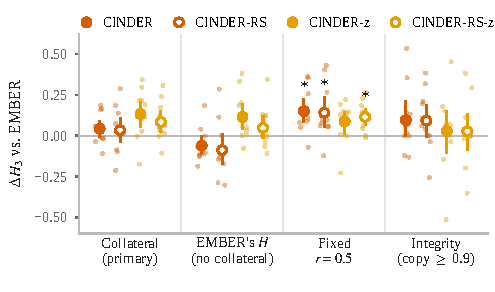
\includegraphics[width=\columnwidth]{figures/results.pdf}
  \caption{Paired test $\Hthree$ difference to \ember{} on the 11 held-out concepts where both edit, by selection rule (integrity-gated: copy $\geq 0.9$, post hoc). Dots: concepts; bars: 95\% bootstrap CI; $*$: Holm $p < 0.05$.}
  \label{fig:results}
\end{figure}

\subsection{Multilingual Erasure}
\label{sec:exp-ml}

\paragraph{One \cinder{} fit replaces eight \ember{} fits}
Counting concepts without an edit as failures, the single \cinderz{} fit (A3z) ties per-language \ember{} (A1; exploratory, non-inferiority not shown): \expnum{0.23} vs.\ \expnum{0.25} strict and \expnum{0.28} vs.\ \expnum{0.25} ungated, \expnum{15--13} in wins and losses ($p = \expnum{0.78}$; Table~\ref{tab:ml}).
Pooling three fit seeds helps \cinderz{} (\expnum{$+0.08$}, $p < 0.001$) but not per-language \ember{}, and the two still tie.

\begin{table}[t]
  \centering
  \small
  \setlength{\tabcolsep}{3.5pt}
  \begin{tabular}{@{}lcccc@{}}
    \toprule
     & A1 & A2 & A3 & A3z \\
    \midrule
    Fits per concept & 8 & 1 & 1 & 1 \\
    Judge calls per concept & \expnum{160} & \expnum{20} & \expnum{20} & \expnum{20} \\
    LLM cost per concept (NIS) & \expnum{.055} & \expnum{.007} & \expnum{.017} & \expnum{.017} \\
    Concepts with a feature (of 38) & \expnum{26} & \expnum{10} & \expnum{21} & \expnum{21} \\
    Score, strict & \expnum{0.25} & \expnum{0.11} & \expnum{0.14} & \expnum{0.23} \\
    Score, ungated & \expnum{0.25} & \expnum{0.14} & \expnum{0.14} & \expnum{0.28} \\
    \bottomrule
  \end{tabular}
  \caption{Multilingual erasure on Llama-3.1-8B-Instruct (38 concepts, 8 languages, fit seed 42, test split; approaches in \S\ref{sec:setup}); concepts without an edit score 0.}
  \label{tab:ml}
\end{table}

\paragraph{A multilingual \ember{} fit rarely accepts the concept}
Where the multilingual \ember{} fit (A2) selects a concept feature, it erases as well as \cinderz{}, but it does so for only \expnum{10} of 38 concepts and \expnum{2} of the 20 held-out ones, against \expnum{21} and \expnum{10} for \cinder{}; counting coverage, \cinderz{} beats it by \expnum{$+0.21$} (\expnum{15--4}, $p = \expnum{0.011}$).
The loss is at the judge more than in the fit: the raw fit contains a lexicon-matching concept feature about as often as \cinder{}'s (\expnum{25--27} vs.\ \expnum{23--28} concepts per seed), but \ember{}'s judge accepts only \expnum{5\%} of those with 3--4 lexicon words, against \expnum{30\%} for \cinder{}'s; re-judged, \twj{} alone lifts the raw fit from \expnum{10} to \expnum{18} concepts, and sharpening alone to \expnum{16} (seed 42, post hoc; \S\ref{app:ml}).

\paragraph{The mean term matters across languages}
Multilingual \cinder{} (A3), whose edit is centred, erases weakly; its uncentred edit (A3z, defined after the development results) adds \expnum{$+0.17$} (\expnum{16 of the 21} edited concepts, $p = \expnum{0.007}$), in the same direction on the 20 pre-registered held-out concepts (\expnum{$+0.19$}, \expnum{7--3}, $p = \expnum{0.064}$).
Across all approaches, erasure is strongest in English, about 0.6 of that in the other Latin-script languages, little in Thai and almost none in Hindi, whose words split into pieces that are rarely concept-only (\S\ref{app:ml}).

%=====================================================================
\section{Embedding-Space Analysis}
\label{sec:analysis}
%=====================================================================

Why does \cinder{} find concepts that \ember{} misses?
We analyze the features before any edit (\expnum{38} concepts, 15 added after the method was frozen; 5 seeds), judge-free wherever possible (\S\ref{app:analyses}).

\paragraph{Sharpening makes the concept pure and valuable}
We seed a sparse feature on each concept's lexicon tokens and run it to its fixed point (Figure~\ref{fig:mechanism}b).
In the raw matrix it drifts toward other rare tokens and ends up only \expnum{24\%} concept-only, although it is among the most valuable features; whitening makes it pure (\expnum{86\%}) but ordinary (\expnum{70th} percentile of feature energies), and sharpening keeps it pure and makes it valuable (\expnum{91st}, higher in \expnum{37 of 38} concepts).
In full fits, a lexicon-matching concept feature appears in \expnum{56\%} of raw, \expnum{49\%} of whitened-only and \expnum{69\%} of sharpened runs, with fewer neutral tokens (\expnum{3.0} vs.\ \expnum{4.5}).
Its nearest neighbour becomes a related topic (magic for Harry Potter) rather than a feature of unrelated rare tokens, and \expnum{97\%} of the raw feature's excess squared norm lies along $\hat\mu_B$ (\S\ref{app:geometry}).

\paragraph{Widths follow the data}
On the sharpened matrix, \ember{}'s 1\% cut stops before the natural tail for \expnum{25 of 38} concepts, and \gs{} widths follow the tail (Spearman \expnum{0.67} vs.\ \expnum{0.27}; mean error \expnum{30} vs.\ \expnum{42} tokens, $p < 0.001$), though they compress its range; \gs{} changes which tokens a feature keeps, not its direction (cosine \expnum{0.97}), and helps only after \cs{} (\S\ref{app:gs}).

\paragraph{The two-way judge recovers concepts lost in the summary}
On 19 concepts, \twj{} accepts the concept or a broader version of it in \expnum{82 of 91} runs, against \expnum{61} for \ember{}'s judge, with \expnum{1 of 110} acceptances unrelated, though most added features are broader than the concept.
On 15 concepts added later, the lexicon path generalizes poorly, whereas showing the judge each token's source word does (TJ with source words \expnum{49}, TJ \expnum{33} of 54 runs; \S\ref{app:twj}).

\paragraph{The gain is not circular}
The concept's page, our sharpening target, contains the sentences whose tokens we score, yet sharpening toward page sentences outside the sample or toward other pages about the concept raises the strict purity of the concept feature as much (\expnum{$+0.06$} vs.\ \expnum{$+0.05$}; Holm $p = \expnum{0.034}$, \expnum{0.081}; pre-registered), while another concept's page destroys it (found in \expnum{2 of 54} runs; \S\ref{app:cs-circ}).

\paragraph{Abstract concepts stay out of reach}
On 13 abstract concepts such as Stoicism and Gothic architecture, the top-ranked feature is specific to the concept in \expnum{0 of 65} runs under both \ember{} and \cs{}, against \expnum{13} and \expnum{23 of 40} for entity concepts; their top features are parent topics and discourse words, perhaps a register they share (untested).
Dilution with adjacent pages hurts \ember{} more than \cs{} (\S\ref{app:robustness}), and features extrapolate only weakly beyond the sample (\S\ref{app:extrapolation}).

\paragraph{The first layer reads the shared mean}
The model's first layer reads \ember{}'s and \cinderz{}'s edits at about twice a random direction, \cinder{}'s at \expnum{1.2$\times$} (Figure~\ref{fig:read}, \S\ref{app:edit}).
The gap is the mean term, read at \expnum{2.9$\times$} a random direction on Gemma and \expnum{20$\times$} on Llama: with $\mu_B$ projected out, \ember{}'s and \cinder{}'s edits are read alike (\expnum{1.31$\times$} vs.\ \expnum{1.32$\times$}).

%=====================================================================
\section{Token-Level Analysis: What an Embedding Edit Removes}
\label{sec:token}
%=====================================================================

Does an embedding edit remove the concept from a word, or the word from the model?
Since the input embedding is where the model first reads a token, we expect an edit to control \emph{access} to the concept through the edited words, at a cost to the words.

\paragraph{Embedding erasure blocks access}
Since only input rows change, efficacy questions that contain none of the edited tokens are answered exactly as before (efficacy \expnum{0.000} in all \expnum{22} configurations checked, including $r = 100$): the knowledge remains in the weights, cut off from the edited words.
At the points our rule selects ($r \approx 1$), efficacy lies close to the floor reached by deleting those words from the questions, above it only for the -z variants.

\paragraph{Removing more costs the words}
At the selected points, about half of the edited words can no longer be read (\expnum{0.49--0.61}, seed 42), and most of the concept-exclusive ones (\expnum{0.65--0.81}), with no significant difference between methods; Table~\ref{tab:examples} shows destruction in free text.
Requiring the words to stay copyable (post hoc) caps efficacy at \expnum{0.06--0.14}; under this constraint \cinder{} removes about twice as much as \ember{} (n.s.), whereas \cinderz{}'s advantage disappears.
On the development concepts, its mean term alone erases more than \cinderz{} at $r \geq 2$ by breaking the prompt (an unrelated question after the word falls below chance), and almost nothing when the words must stay copyable (\S\ref{app:mean}).

\paragraph{A nonce-like edit is only partly reachable}
An erased word should behave like a nonce, copyable but meaningless; a learned edit that pushes each edited word toward its nonce's behaviour (post hoc) removes \expnum{2--3$\times$} as much as copy-gated \ember{} while keeping the words copyable, but reaches a substantial nonce floor in only \expnum{2} of 12 concepts (seed 42; \S\ref{app:nonce}).
Figure~\ref{fig:integrity} (\S\ref{app:eval}) traces this trade-off along the edit-size grid.

\begin{table}[t]
  \centering
  \small
  \setlength{\tabcolsep}{3pt}
  \begin{tabular}{@{}P{2.0cm}P{2.45cm}P{2.45cm}@{}}
    \toprule
    Prompt & $\delta = 1$ ($r \approx 0.6$) & $\delta = 200$ (selected by $H$) \\
    \midrule
    Who is Prince \textbf{Harry}, and who is his wife? & \textit{Prince Harry is the second son of King Charles III [\dots] His wife is Meghan Markle} & \textit{Prince was an American singer, songwriter [\dots] Prince's wife was Mayte} \\
    \addlinespace
    What country does the toy company \textbf{Lego} come from [\dots]? & \textit{Lego comes from Denmark.} & \textit{Please provide me with the name of the toy company!} \\
    \bottomrule
  \end{tabular}
  \caption{Gemma-2-2B-it after erasing Harry Potter with \ember{} (seed 42) at a moderate strength and at the strength \ember{}'s score selects. Edited tokens, both from the Harry Potter feature, are in bold.}
  \label{tab:examples}
\end{table}

%=====================================================================
\section{Related Work}
\label{sec:related}
%=====================================================================

\paragraph{Concept Erasure and Its Evaluation}
Unlearning methods optimize a forget objective \citep{eldan2023harry,li2024wmdp,ashuach2026crisp} or edit the parameters that store the concept \citep{gurarieh2025precise,shafran2026constructing,suslik2026ember}; in both, erasure is often undone by relearning \citep{deeb2024unlearning}, adversarial prompts \citep{lynch2024eight} or another format \citep{ye2025formindependent,hong2025intrinsic}.
Knowledge editing tests specificity on \emph{neighborhood} prompts that share surface form with the edit \citep{meng2022locating}; our collateral term brings this idea to embedding erasure, and our nonce reference follows the \emph{wug} test \citep{berko1958child}.

\paragraph{Sparse Dictionaries and Their Interpretation}
Sparse factorizations recover interpretable parts of data \citep{lee1999nmf,hoyer2004nmf} and of model activations \citep{bricken2023monosemanticity,huben2024sparse,gao2025scaling}, with the sparsity allocation shaping what is found \citep{makhzani2014ksparse,bussmann2024batchtopk}; their features are commonly named by an LLM \citep{bills2023language,paulo2024automatically}, whose verbalized confidence is poorly calibrated \citep{xiong2024can}.

\paragraph{Geometry of Token Embeddings}
Embedding spaces are anisotropic \citep{ethayarajh2019contextual,mu2018allbutthetop}, rare tokens degenerate \citep{gao2019representation}, and whitening improves semantic similarity \citep{su2021whitening}; INLP and LEACE \citep{ravfogel2020null,belrose2023leace} also whiten, but to remove a concept from representations, whereas we whiten to find it in the weights.

\paragraph{Multilingual Knowledge and Unlearning}
Multilingual LMs encode language identity in a few dominant directions \citep{chang2022geometry,libovicky2020language} and share conceptual knowledge across languages \citep{wendler2024llamas}, yet unlearning in one language often fails to carry over \citep{choi2024crosslingual,lu2025learn}.
For embedding erasure the failure is structural, since an edit to English rows cannot reach another script's tokens, and \citet{suslik2026ember} leave other languages to future work.

%=====================================================================
\section{Conclusion}
\label{sec:conclusion}
%=====================================================================

\ember{} often misses concept features because concept tokens share a common direction with other rare tokens.
\cinder{} sharpens the embedding matrix toward the concept, lets each feature find its width and verifies features both ways, and one multilingual fit covers eight languages at an eighth of the judge calls.
Under an evaluation that stops rewarding destroyed tokens, \cinder{} reaches more concepts and, at moderate edit size, removes more, and embedding erasure blocks access to a concept through its words.
Where the edited words must stay usable, we recommend \cinder{}'s centred edit: \cinderz{} scores higher only where the evaluation does not require the words to stay readable (\S\ref{sec:token}).

%=====================================================================
\section*{Limitations}
%=====================================================================

\paragraph{Model and language coverage}
Single-language results use one small model (Gemma-2-2B-it) in English, and multilingual results use one model (Llama-3.1-8B-Instruct) with a 4-bit quantized transformer and fp16 embeddings.
Whether the findings transfer to other models remains to be tested.

\paragraph{Abstract concepts}
Concepts that lie between broader topics, such as Stoicism or Gothic architecture, yield no concept-specific embedding feature under \ember{} or \cinder{} (\S\ref{sec:analysis}); embedding-level erasure, with either method, does not reach them.

\paragraph{Embedding edits in isolation}
We evaluate embedding edits on their own, not ensembled with MLP-based methods as \ember{} recommends, and we do not test robustness to relearning, \ember{}'s main strength.
Whether relearning robustness also depends on the edit size ($r \approx 1$ vs.\ $r \approx 100$) is an open question.

\paragraph{Evaluation material}
Efficacy and collateral are multiple-choice accuracies, and collateral is lenient, since the options and context can rescue a damaged word.
Collateral questions, neutral prompts and free-text labels were written and checked by LLM agents, whose blind spots may be correlated, and no human spot check was done; non-English questions are machine-translated.

\paragraph{Multilingual evaluation}
The multilingual study follows \ember{}'s protocol (its $\delta$ grid and metrics, with perplexity in place of Alpaca) and has no collateral term, so, like the standard protocol, it cannot tell erasing a concept from destroying its words.
On Gemma's three development concepts, the mean term that \cinderz{} and \ember{} add to their edits erases mostly by damaging the prompt (\S\ref{sec:token}), so part of multilingual \cinderz{}'s gain over \cinder{}, and of every approach's score, may be such damage; the mean-only test was not repeated on Llama.

\paragraph{Statistical power}
With 11--12 held-out concepts as the unit of analysis, differences below about 0.08 are hard to resolve, and several supporting analyses were defined after the primary result was known; we label them post hoc.

\paragraph{Sharpening target}
Contrastive Sharpening uses the concept's own Wikipedia page as its target, which overlaps the concept sentences. Targets disjoint from the sample keep the feature-level gains (\S\ref{sec:analysis}), but the erasure experiments use the page target, and $\eta$ and $\gamma$ were chosen with it.

%=====================================================================
\section*{Ethical Considerations}
%=====================================================================

\cinder{} is designed to remove hazardous, private or copyrighted knowledge more reliably.
Like other editing techniques, it carries a dual-use risk: an effective erasure method could be used to suppress legitimate information.
Our evaluation findings also carry a caution: embedding-level erasure, as commonly evaluated, can appear effective while only blocking access through specific words and damaging their other meanings, so it should not be relied on alone to remove dangerous knowledge.

%=====================================================================
\section*{AI Disclosure and Reflection}
%=====================================================================

The research questions, hypotheses and main ideas of this work are our own; we used AI tools to support them, not to replace them.
We used Claude Code (Anthropic) as a research assistant: to brainstorm and critique our ideas, to implement and debug the experiment code, and to scale the experiments to 38 concepts, several seeds and eight languages on the cluster.
In the final experimental stages, once we were satisfied with their direction, we let it make routine decisions within the plan we had set, and reviewed them afterwards.
It also helped draft and revise this report; we read every part of it, marked what to change, and set its style, its framing and the negative results it reports.
LLMs also produced part of the evaluation material: Claude agents wrote and checked the collateral questions and neutral prompts and labelled features and free-text answers without seeing the method (\S\ref{sec:setup}), and Gemini~3.5 Flash-Lite generated and verified the questions of the 20 new multilingual concepts.
Within the method, Gemini~3.5 Flash-Lite is the feature judge, the lexicon generator and the coherence judge (\ember{} used Gemini~2.5 Flash-Lite).
We take full responsibility for every claim in the paper.

\paragraph{Reflection}
The assistant was most useful for implementation and scale: it let us test each idea on many concepts and seeds rather than a few examples.
The ideas behind \cinder{}, however, came from working with the data by hand: we wrote Jupyter notebooks with the assistant's help, ran them ourselves, inspected the features and the evaluations, and experimented.
We found no substitute for this, and our impression is that the assistant could not have proposed these directions on its own.
It was least reliable where judgement was needed.
It stated findings with more confidence than it had, so we asked it to give a confidence level with each claim; its drafts were dense; numbers drifted from the result files, and two audits of the text against them corrected about 40 claims; and it sometimes acted before we had agreed, starting an analysis we had only discussed or editing text we had asked only to discuss.
We therefore kept the decisions with us and checked its claims against the code and the results.


\bibliography{references}

\appendix
%=====================================================================
\section{\ember{}: Reproduction Details}
\label{app:ember}
%=====================================================================

\paragraph{Sparse MF}
We follow \ember{}'s App.~A.1.
Given $A \in \R^{d \times n}$, alternating least squares updates $Y \leftarrow (Z^{\top}Z + \lambda I)^{-1}Z^{\top}A$ and $Z \leftarrow AY^{\top}(YY^{\top} + \lambda I)^{-1}$ with ridge $\lambda = 10^{-4}$.
After each $Y$ update the sparsity rule is applied to the dense $Y$ (row sparsity: the top $\lceil s\,n \rceil$ entries of each row by magnitude, $s = 0.01$), and each row of $Y$ is rescaled to unit norm with the scale absorbed into $Z$.
$Z$ and $Y$ start from i.i.d.\ $\mathcal N(0,1)$ draws; we stop when the relative error improves by less than $10^{-4}$ for 200 iterations and the support changes in fewer than 0.5\% of its entries, or after 20{,}000 iterations.
$k = 100$ on Gemma-2-2B-it ($d = 2304$) and $k = 200$ on Llama-3.1-8B-Instruct ($d = 4096$).
Embeddings are the input embedding rows scaled by $\sqrt d$ for Gemma, as the model uses them.

\paragraph{Data}
\ember{}'s 18 concepts: Ancient Rome, Artificial Intelligence, Baseball, Cannabis, COVID-19 pandemic, Culture of Greece, Gambling, Golf, Gun, Halloween, Harry Potter, Heroin, Nazism, Pornography, Republic of Ireland, Uranium, Valentine's Day, World War II.
$\Sc$ holds 300 sentences sampled from the concept's Wikipedia page and $\Sn$ 300 sentences from random English Wikipedia pages (sampling seed 42); for Harry Potter $|\vs| = 4{,}780$.
Questions follow \ember{}: 50 validation and 50 test multiple-choice questions per concept and per similar domain, and MMLU \citep{hendrycks2021mmlu}.
The 20 additional concepts are listed in App.~\ref{app:ml}.

\paragraph{Feature selection}
The 20 features with the largest $\rho$ (Eq.~\ref{eq:rho}) and $\rho > 2$ go to the judge, which uses \ember{}'s two prompts (its Figures 4--5) on each feature's top 20 concept-labelled tokens and accepts at confidence $\geq 0.85$.
Our judge is Gemini~3.5 Flash-Lite; \ember{} used Gemini~2.5 Flash-Lite.
Re-judging 230 candidates flipped 0.4\% of decisions.

\paragraph{Fidelity}
On \ember{}'s protocol our reproduction reaches concept, similar-domain and MMLU accuracy of \expnum{48.4}, \expnum{83.2} and \expnum{55.1}, against \expnum{52.1}, \expnum{84.6} and \expnum{53.6} in the paper's Table~6.
Tuning with Alpaca coherence inside the $\delta$ grid, as the paper does, gives the same $\delta$ and result as our cheaper MMLU gate on Harry Potter ($H = \expnum{0.727}$ vs.\ \expnum{0.726}).
In an earlier phase we found that a 4-token answer budget in the original multiple-choice scorer counted many correct answers as wrong at large edit strengths, inflating \ember{}'s efficacy. All erasure numbers here use the repaired scorer, except the cross-lingual leakage of the first study (App.~\ref{app:ml}), which we report with the original scorer and with unparseable answers dropped.

\paragraph{Why the protocol misses token destruction}
Over the \expnum{344} points of the first erasure run (\ember{} and six intermediate variants on 14 concepts, 8 strengths each, seed 42), MMLU never falls below \expnum{0.93} of the unedited model, so the 0.9 gate never rejects a strength, and Alpaca coherence stays at or above \expnum{0.92} at every selected point; the similar-domain questions avoid the edited words.
We wrote 20 neutral prompts per development concept, most using an edited word in another sense (Prince Harry, Caesar salad) and a few on adjacent topics with no edited word, and compared each greedy answer with the unedited model's.
At $\delta = 200$, \ember{} breaks \expnum{12}, \expnum{3} and \expnum{7} of 20 on Harry Potter, Ancient Rome and Valentine's Day (seeds 42, 44 and 42), and \cinder{} \expnum{9}, \expnum{12} and \expnum{9}; at $\delta = 1$, both break \expnum{0--1} on each.
$\delta = 200$ is \ember{}'s selected strength on Harry Potter; for \cinder{}, which selected $\delta = 2$ there, it is a stress test.

%=====================================================================
\section{Contrastive Sharpening: Details}
\label{app:cs}
%=====================================================================

\subsection{Construction}

\paragraph{Background}
The background is the set of token types in a sample of English Wikipedia, each type counted once (\expnum{107{,}472} types for Gemma), so that a direction is loud in the background because many \emph{different} tokens use it, not because a few frequent ones do.
We compute its mean $\mu_B$ and covariance $\Sigma_B = Q\Lambda Q^{\top}$ once per model.
The ridge $\varepsilon = 10^{-4}\cdot\operatorname{mean}(\Lambda)$ only damps the smallest eigenvalues.

\paragraph{Target}
The sharpening target is the set of token types of the concept's English Wikipedia page ($m = \expnum{3{,}124}$ for Harry Potter), whitened with Eq.~\ref{eq:whiten}.
$\eta = 0.05$ and $\gamma = 1$ were chosen by a judge-free sweep on Harry Potter, Ancient Rome and Valentine's Day: each of five values of $\eta$ was ranked by concept-vs-neutral AUC, concept-only purity of the top feature, concept-token coverage and $\rho_{\max}$, and the lowest mean rank won.
$\eta = 1$ is whitening only; $\gamma$ sets how strongly enriched directions are stretched.

\paragraph{Exact inverse}
In column form, $\mathbf x_t = T(\e_t - \mu_B)$ with $T = S_\eta^{\gamma/2}W$, which is invertible because $S_\eta \succeq \eta I$ and $W \succ 0$.
If sparse MF gives $\mathbf x_t \approx \sum_i Y_{i,t}\tilde\z_i$, then $\e_t - \mu_B \approx \sum_i Y_{i,t}\,T^{-1}\tilde\z_i$: the same coefficients reconstruct the original embedding with the mapped-back dictionary $\z_i = T^{-1}\tilde\z_i = W^{-1}S_\eta^{-\gamma/2}\tilde\z_i$, and the mean cancels in any difference.
Every erasure run checks numerically that the transformed embedding rows equal the factorized matrix columns before editing.

\subsection{Why sharpening finds the concept}

Let $M = \frac1m\sum_j \tilde{\mathbf u}_j\tilde{\mathbf u}_j^{\top} = P\,\mathrm{diag}(\lambda_j)\,P^{\top}$ be the whitened second moment of the target, so that $S_\eta = P\,\mathrm{diag}(g_j)\,P^{\top}$ with $g_j = (1-\eta)\lambda_j + \eta$.

\begin{proposition}
\label{prop:cs}
(i) The eigenvalues of $M$ are the generalized eigenvalues of the pair $(\Sigma_C + \bm\delta\bm\delta^{\top},\, \Sigma_B + \varepsilon I)$, i.e.\ the stationary values of the ratio $R$ of Eq.~\ref{eq:rayleigh}, attained at $\mathbf v_j = W\mathbf p_j$.
(ii) For any set of tokens with whitened second moment $G$, the second moment of the sharpened tokens along $\mathbf p_j$ is $g_j^{\gamma}\,\mathbf p_j^{\top}G\,\mathbf p_j$.
In particular, background tokens, for which $G = I$ up to $\varepsilon$, carry the same energy along every direction after whitening and $g_j^{\gamma}$ after sharpening, and the target's own energy along $\mathbf p_j$ becomes $g_j^{\gamma}\lambda_j \approx (1-\eta)^{\gamma}\lambda_j^{1+\gamma}$ for $\lambda_j \gg \eta$.
\end{proposition}

\begin{proof}[Proof sketch]
(i) $\mathbf p^{\top}M\mathbf p = \mathbf p^{\top}W(\Sigma_C + \bm\delta\bm\delta^{\top})W\mathbf p$, since the target's second moment around $\mu_B$ is $\Sigma_C + \bm\delta\bm\delta^{\top}$; with $\mathbf v = W\mathbf p$ and $\mathbf p^{\top}\mathbf p = \mathbf v^{\top}W^{-2}\mathbf v = \mathbf v^{\top}(\Sigma_B + \varepsilon I)\mathbf v$, the Rayleigh quotient of $M$ equals $R(\mathbf v)$.
(ii) $S_\eta^{\gamma/2}\mathbf p_j = g_j^{\gamma/2}\mathbf p_j$, so $\mathbf p_j^{\top}S_\eta^{\gamma/2}GS_\eta^{\gamma/2}\mathbf p_j = g_j^{\gamma}\,\mathbf p_j^{\top}G\mathbf p_j$.
\end{proof}

Since the error that a sparse-MF feature removes is the energy of its support along it, the proposition says which directions sparse MF will find profitable.
In the raw matrix they include the mean direction that rare tokens share, so a concept's rare tokens are grouped with other rare tokens.
After whitening, all background directions are equally profitable, so the concept's tokens form a pure cluster of ordinary value; whitening alone finds a concept feature less often than the raw matrix (on Harry Potter it merges the concept with magic).
After sharpening, they are ordered by the concept-to-background ratio, raised to the power $1+\gamma$ for the concept's own tokens.
Two further facts make this precise.
First, \ember{}'s alternating fit depends on $A$ only through the token Gram matrix $K = A^{\top}A$: with $G_Y = YY^{\top}+\lambda I$, the dictionary update gives $Z^{\top}Z = G_Y^{-1}YKY^{\top}G_Y^{-1}$ and $Z^{\top}A = G_Y^{-1}YK$, so the dense solve, the masks and the error are functions of $K$ (verified numerically: identical supports for $A$ and $QA$, $Q$ orthogonal).
Under \cs{} with $\gamma = 1$, $K$ becomes a \emph{page kernel}, $K(s,t) = (1-\eta)\frac{1}{m}\sum_{j\in\text{page}} k(s,j)\,k(t,j) + \eta\,k(s,t)$, with $k$ the background-Mahalanobis inner product: two tokens are similar when they resemble the same tokens of the concept page.
Second, with the other features fixed, the best feature on a support $S$ of fixed size lowers the error by $\sigma_1(R_S)^2 = \big(\sum_{t\in S}\|\mathbf r_t\|^2\big)\,\kappa(S)$, the support's energy times its coherence $\kappa(S) \in [1/|S|, 1]$.
A concept can therefore fail in two ways: it is \emph{impure} if other tokens project more strongly along its best direction (the raw case, where rare tokens share $\hat\mu_B$), or \emph{unprofitable} if its energy times coherence is below what other directions offer (the whitened-only case).
Across concepts the largest gain is $g_1 = \expnum{15.7}$ (median; range \expnum{10.9--29.3}), and \expnum{870} of 2{,}304 directions have $g_j > 1$.

\paragraph{Decomposition}
Medians over 38 concepts $\times$ 5 seeds, row sparsity:

\begin{center}
\footnotesize
\setlength{\tabcolsep}{2pt}
\begin{tabular}{@{}lccccc@{}}
\toprule
 & raw & $\perp\hat\mu_B$ & centred & whit. & \cs{} \\
\midrule
Concept found (\% runs) & \expnum{56} & \expnum{61} & \expnum{59} & \expnum{49} & \expnum{69} \\
Its neutral tokens & \expnum{4.5} & \expnum{4.5} & \expnum{4.5} & \expnum{4.0} & \expnum{3.0} \\
Its $\|\z\|^2$ percentile & \expnum{86} & \expnum{66} & \expnum{41} & \expnum{54} & \expnum{58} \\
Seeded: purity & \expnum{.24} & \expnum{.27} & \expnum{.04} & \expnum{.86} & \expnum{.86} \\
Seeded: value pct. & \expnum{100} & \expnum{97} & \expnum{100} & \expnum{70} & \expnum{91} \\
SVD rank matching & \expnum{4} & \expnum{22} & \expnum{4} & \expnum{66} & \expnum{49} \\
\bottomrule
\end{tabular}
\end{center}

\noindent The seeded feature starts on the concept's lexicon tokens and alternates between the top singular vector of its support and the top tokens along it until the support repeats.

\subsection{Is the gain circular?}
\label{app:cs-circ}
\label{app:cs-sens}

\paragraph{Design}
18 \ember{} concepts, seeds 42--44, row sparsity (global sparsity as a secondary analysis), everything fixed except the sharpening target, pre-registered before any new fit.
Targets: the page (default); \emph{disjoint}, page sentences that are not near-duplicates of any sampled sentence; \emph{related}, four other Wikipedia pages about the concept, taken by rule from the page's ``Main'', ``Further'' and ``See also'' links and size-matched; a random page subset as large as \emph{disjoint}; the leak-free control (page minus every token of $\vs$); and \emph{wrong}, the page of an unrelated concept.
A token is \emph{strict} if it is concept-only and either a lexicon word or occurs at least twice in $\Sc$ and is at least ten times more frequent there than in Wikipedia.

\paragraph{Results}
Strict purity of the best concept feature (raw \expnum{.568}): page \expnum{$+.052$} ($p = \expnum{.088}$), disjoint \expnum{$+.060$} (\expnum{.003}; Holm \expnum{.034}), related \expnum{$+.062$} (\expnum{.009}), page subset \expnum{$+.046$}, leak-free \expnum{$-.064$} (n.s.), wrong \expnum{$-.445$} ($p < 10^{-4}$).
Separability of strict and neutral tokens (AUC, raw \expnum{.576}): page \expnum{$+.055$} (17 of 18 concepts), related \expnum{$+.041$} (17 of 18), disjoint \expnum{$+.037$} (15 of 18); on tokens absent from the target, related still gives \expnum{$+.034$} ($p = \expnum{.0003}$).
With the wrong page the concept feature is found in \expnum{2 of 54} runs (raw \expnum{39}).
The coverage measure used to choose $\eta$ rises only with the page target (\expnum{$+.033$}) and falls with the disjoint and related ones, so it was the circular quantity.
The target also steers which side of the concept is amplified: for Harry Potter, the page keeps the proper-name feature, while the disjoint and related targets yield a ``magic'' feature, both ranked first.
Under global sparsity the purity gain disappears for every target, page included, while the separability gains remain.

\paragraph{Sensitivity to $\eta$ and $\gamma$}
On the 15 concepts outside the tuning set (page target, 3 seeds), every setting of $\eta \in \{0.05, 0.2, 0.5\}$ and $\gamma \in \{0.5, 1, 2\}$ beats the raw matrix on strict purity, separability and $\rho$-rank; the default ranks 6th of 9, $\gamma = 2$ is slightly better (\expnum{$+.024$} purity), and $\gamma = 0.5$ is worst on every measure.

\subsection{Models with a larger embedding dimension}
\label{app:cs-llama}

\paragraph{The question}
$S_\eta$ is estimated from the $m$ token types of one page.
On Llama-3.1-8B ($d = 4096$), 15 of the 18 English pages have $m < d$ (median $m/d = \expnum{0.77}$; Gemma \expnum{1.29}), so $(1-\eta)M$ has a null space that sharpening shrinks to $\eta^{\gamma/2}$.

\paragraph{Rank is not the problem}
The fitted features put under \expnum{0.5\%} of their mapped-back norm into these floor directions; the three Llama pages with $m > d$ fail like the others; and Gemma pages cut below $d$, or Gemma's own pages with $m < d$, work as before.

\paragraph{Noise is}
Only about \expnum{12} eigenvalues of Llama's whitened page moment exceed the largest eigenvalue of the same moment computed from $m$ random background types (Gemma: \expnum{74}), and in the noise-dominated bulk each page token's own outer product supplies about half of its sharpened energy (predicted $d/(d+m)$; measured median \expnum{0.54}, correlation \expnum{0.99} across 36 model--concept pairs).
Since almost every concept-only token of $\vs$ is on the page, sharpening then amplifies page membership rather than the concept: on Llama, \expnum{92\%} of features pass $\rho \ge 2$ (\ember{} \expnum{32\%}), their words are close to incoherent, and the concept feature falls from a $\rho$-rank of about \expnum{10} to about \expnum{38} ($p = \expnum{10^{-4}}$, 18 concepts $\times$ 3 seeds).
No $\eta \in [0.05, 0.5]$ or $\gamma \in \{0.5, 1\}$ changes this, since the echo sits in the bulk, not on the floor.

\paragraph{Rule}
Sharpen only the resolvable directions, $S = I + \sum_{j:\lambda_j > \hat\lambda_{\text{edge}}} \big((1-\eta)\lambda_j + \eta - 1\big)\,\mathbf p_j\mathbf p_j^{\top}$, with $\hat\lambda_{\text{edge}}$ the largest eigenvalue of the random-type moment (the Marchenko--Pastur edge $(1+\sqrt{d/m})^2$ is a close closed form).
On Llama this gives a concept-feature rank of about \expnum{5} against \expnum{10} for \ember{} ($p = \expnum{0.015}$) with \ember{}'s coherence, though no better than whitening alone; on Gemma it keeps 47--98 directions and changes nothing.
Pooling the concept's text over eight languages raises the number of resolvable directions to about \expnum{85}, which, with the same rule, also works (rank \expnum{4.5}).

%=====================================================================
\section{Global Sparsity: Details}
\label{app:gs}
%=====================================================================

\begin{algorithm}[t]
\caption{Sparse MF with Global Sparsity (one iteration)}
\label{alg:gs}
\small
\begin{algorithmic}[1]
\Require $A \in \R^{d\times n}$, $Z \in \R^{d\times k}$, budget $K = \lceil s\,n\rceil k$, floor $m_{\min}$, cap $m_{\max}$
\State $Y^{\mathrm{d}} \gets (Z^{\top}Z + \lambda I)^{-1}Z^{\top}A$ \Comment{dense update}
\State $s_{ij} \gets |Y^{\mathrm{d}}_{ij}| \,/\, \|Y^{\mathrm{d}}_{i,:}\|_2$ \Comment{scale-free share}
\State $\mathcal S \gets$ the top $m_{\min}$ entries of every row by $s_{ij}$
\State add the remaining entries in decreasing $s_{ij}$, skipping rows with $m_{\max}$ entries, until $|\mathcal S| = K$
\State $Y \gets Y^{\mathrm{d}} \odot \mathbb 1_{\mathcal S}$; rescale rows of $Y$ to unit norm, absorb scales in $Z$
\State $Z \gets AY^{\top}(YY^{\top} + \lambda I)^{-1}$
\end{algorithmic}
\end{algorithm}

\paragraph{Algorithm}
Algorithm~\ref{alg:gs} replaces \ember{}'s per-row top-$k$ step; everything else is unchanged.
The budget equals \ember{}'s total ($1\%$ of all entries); the floor is $0.2\%$ and the cap $3\%$ of the tokens per feature ($m_{\min} = 10$, $m_{\max} = 144$ on Harry Potter).
The cap exists for generic features; no concept feature reached it in \expnum{190} runs over \expnum{38} concepts (widest: Culture of Greece, \expnum{120} of 156 tokens).

\paragraph{Variants}
All five rules below share the matrix, the budget and the fitting loop.

\begin{center}
\small
\setlength{\tabcolsep}{3pt}
\begin{tabular}{@{}lP{2.9cm}P{2.1cm}@{}}
\toprule
Rule & Support & Role \\
\midrule
RS-1\% & top 1\% of each row & \ember{} \\
RS-2\% & top 2\% of each row & more tokens, no reallocation \\
GS-norm & global top-$K$ of $|y_{ij}|/\|\mathbf y_i\|$ & \cinder{} \\
GS-gain & global top-$K$ of $|y_{ij}|\,\|\z_i\|$ & favours loud features \\
GS-entropy & width $\propto$ effective support $e^{H(\mathbf y_i)}$ & ablation \\
\bottomrule
\end{tabular}
\end{center}

\noindent An $\ell_1$-penalized variant (the Lasso, \citealt{tibshirani1996lasso}), tuned to the same number of nonzeros, never produced a clean Ancient Rome feature in 5 seeds and was dropped.

\paragraph{Results}
On the sharpened matrix, 18 concepts $\times$ 5 seeds (cap 5\% in this sweep):

\begin{center}
\footnotesize
\setlength{\tabcolsep}{2pt}
\begin{tabular}{@{}lccccc@{}}
\toprule
 & RS-1\% & RS-2\% & GS-norm & GS-gain & GS-ent. \\
\midrule
Width & 43--52 & 86--104 & 15--113 & 9--143 & 25--121 \\
Seed MAD & 0 & 0 & 4.1 & 8.1 & 7.9 \\
Clean runs (/90) & 75 & 31 & 76 & 55 & 61 \\
Neutral share & 5.8\% & 8.2\% & 5.6\% & 8.0\% & 8.2\% \\
Seed Jaccard & .719 & .726 & .735 & .717 & .733 \\
\bottomrule
\end{tabular}
\end{center}

\noindent MAD: mean absolute deviation of a concept's width across seeds. A run is clean when its concept feature has at most five neutral tokens.
Only GS-norm adapts the width per concept while staying as clean and stable as \ember{}'s rule.
This sweep used a 5\% cap; with the current 3\% cap, concept widths range over \expnum{21--114} tokens (concept means).

\subsection{Widths and the Natural Tail}
\label{app:gs-tail}
We use the saved fits of 38 concepts $\times$ 5 seeds (\ember{}; \cs{} with row sparsity; \cs{}+\gs{}; raw \gs{}; \cs{} with 2\% row sparsity), 950 fits in all.
\emph{Dense re-solve.} With the saved dictionary fixed, $Y' = (Z^{\top}Z+\lambda I)^{-1}Z^{\top}A$ equals $Y$ on the support in every fit (maximum error \expnum{$2.2\cdot10^{-6}$}), and every \gs{} support is exactly the set of tokens whose share exceeds a single threshold per fit.
\emph{Natural tail.} Along the dense ranking of the concept feature (identified by lexicon hits), a token is \emph{page-enriched} if it occurs in $\Sc$ and is at least 20 times more frequent there than in Wikipedia; the natural tail $T$ is the first rank at which fewer than half of the next 20 tokens are page-enriched, fixed before any width statistic was computed.
\emph{Results.} On the sharpened matrix the median $T$ is \expnum{69} tokens against a row-sparse width of \expnum{47}; the 1\% cut is short for \expnum{25}, long for \expnum{8} and about right for \expnum{5} of 38 concepts (raw matrix: \expnum{15}, \expnum{15}, \expnum{8}).
Doubling the budget moves $T$ by \expnum{$+3$} tokens (rank correlation \expnum{0.96}).
\gs{} widens \expnum{26} of the \expnum{28} features cut short; its width correlates with $T$ at \expnum{0.67 [0.42, 0.84]} against \expnum{0.27} for the row-sparse width, with mean error \expnum{30} vs.\ \expnum{42} tokens ($p = \expnum{0.0009}$).
This holds for all 45 non-degenerate definitions of the tail in a grid of 72, but \gs{} compresses the range (slope \expnum{0.30}): it overshoots narrow concepts by \expnum{24} tokens and undershoots broad ones by \expnum{44} (e.g., Buddhism \expnum{100} vs.\ \expnum{182}).
\emph{Stability.} The width's seed deviation is \expnum{4} tokens when the same feature is identified (\expnum{7.7} overall), and the width is unrelated to the feature's index ($\rho = \expnum{-0.004}$).
\emph{Breadth.} \gs{} width does not correlate with counts of concept tokens (\expnum{0.05}); that count ranks concepts exactly like $|\vs|$, since $\Sn$ is shared.
\emph{Direction.} The \gs{} and row-sparse concept features have cosine \expnum{0.97} (within seed noise); raw and sharpened features, mapped back, only \expnum{0.75}.
\emph{\gs{} needs \cs{}.} On the raw matrix, the width that \gs{} adds beyond the row-sparse width is \expnum{16\%} neutral (against \expnum{7\%} for its first 47 tokens), and raw \gs{} does not track $T$ better than row sparsity ($p = \expnum{0.39}$).
Under \gs{} the concept feature ranks first by $\rho$ less often than under \cs{} with row sparsity (\expnum{18\%} vs.\ \expnum{38\%} of runs), although its wider support holds more concept tokens (\expnum{54} vs.\ \expnum{41.5}).

%=====================================================================
\section{Two-Way Judge: Details}
\label{app:twj}
%=====================================================================

\paragraph{Lexicon}
Once per concept, before any feature is judged, the LLM receives:
\begin{quote}
\small\itshape
Given the concept `\{concept\}', list the \{n\} words most strongly associated with it. Rules: Start with the concept's own name and its basic word forms when they are single words [\dots]. Then the entities, people, places, objects, actions and terms that an ordinary person with general knowledge would immediately connect to this concept. Prefer well-known words over expert or niche terminology. Every word must be specific to this concept: avoid words that fit its broader category just as well (e.g.\ for `World War II' not `war', `battle' or `soldier'). Single words, lowercase, no duplicates or mere plural variants. Return ONLY a JSON list of \{n\} strings.
\end{quote}
with $n = 20$.
The prompt's examples name four concepts (Culture of Greece, Ancient Rome, Artificial Intelligence, World War II), which we exclude when evaluating the judge.
In the multilingual pipeline the same call returns 20 words in each of the eight languages.

\paragraph{Feature words}
For each of a feature's top tokens we take the word in $\Sc$ that most often produces it (\textit{ffindor} $\to$ \textit{gryffindor}), lowercase and deduplicate the words, and keep the first 20; EJ@$t$ accepts when at least $t$ of them are lexicon words.

\paragraph{Variants}

\begin{center}
\small
\setlength{\tabcolsep}{3pt}
\begin{tabular}{@{}lP{4.3cm}@{}}
\toprule
Rule & Accepts when \\
\midrule
TJ & \ember{}'s two-stage judge accepts \\
WJ & TJ, shown each token's source words \\
WJ+share & WJ, and the concept share is $\geq 0.5$ \\
EJ@$t$ & $\geq t$ lexicon words among the feature's words \\
\twj{} & TJ $\vee$ EJ@5 \\
\twj{}-R & WJ+share $\vee$ EJ@4 \\
\bottomrule
\end{tabular}
\end{center}

\paragraph{Labelled evaluation}
Every rule scored every candidate feature of the \cs{}+\gs{} fits (23 concepts $\times$ 5 seeds, 7{,}105 candidates).
Every feature accepted by some rule was labelled, without seeing the rules' decisions, as P (specific to the concept), B (broader or adjacent, e.g.\ nuclear physics for Uranium) or N (unrelated).
Excluding the four prompt-example concepts leaves 19 concepts and 95 runs; a run is hit when an accepted feature is positive.

\begin{center}
\small
\setlength{\tabcolsep}{2.5pt}
\begin{tabular}{@{}lcccccc@{}}
\toprule
 & \multicolumn{3}{c}{P only} & \multicolumn{3}{c}{P + B} \\
\cmidrule(lr){2-4}\cmidrule(l){5-7}
Rule & Prec. & Rec. & Hit/72 & Prec. & Rec. & Hit/91 \\
\midrule
TJ & .85 & .69 & 60 & 1.00 & .41 & 61 \\
WJ & .56 & .81 & 61 & .77 & .55 & 66 \\
EJ@5 & .74 & .64 & 64 & .99 & .43 & 81 \\
\twj{} & .71 & .77 & 67 & .99 & .54 & 82 \\
\twj{}-R & .61 & .90 & 71 & .91 & .68 & 84 \\
\bottomrule
\end{tabular}
\end{center}

\noindent Recall counts only positives that some rule accepted.
The threshold $t = 5$ was chosen on this set.
On the 15 concepts added after the prompt was fixed, EJ@5 does not generalize (precision \expnum{0.46}, recall \expnum{0.26}) and \twj{} falls to \expnum{0.53}/\expnum{0.56}, whereas TJ $\vee$ WJ+share keeps precision \expnum{0.71} and recall \expnum{0.89} (\expnum{49} of 75 runs hit, against \expnum{33} for TJ).
In erasure the two judges perform the same.
\expfill{Final judge comparison table on the held-out concepts, and a per-concept list of TJ's wrong rejections.}

\paragraph{Cost}
TJ makes two LLM calls per candidate feature (up to 20 per run).
The lexicon path makes one call per concept, shared by all seeds and fits, and its matching is deterministic, so its decisions are reproducible and free to recompute after any change to the factorization.

%=====================================================================
\section{Centred and Uncentred Edits}
\label{app:edit}
%=====================================================================

\paragraph{Read strength}
The first thing the model does with an embedding is normalize it and project it into queries, keys and values.
For a unit direction $\mathbf u$ we define its read strength as $\big\|[W_Q; W_K; W_V]\,(\mathbf g \odot \mathbf u)\big\|$, with the layer-0 attention projections stacked and $\mathbf g$ the layer-0 RMSNorm scale, relative to the mean over 500 random unit directions; for Llama we also stack the MLP's gate and up projections, as the multilingual study did.
For a method we take the median over its edited tokens' directions $\cvec_t / \|\cvec_t\|$.

\begin{figure*}[t]
  \centering
  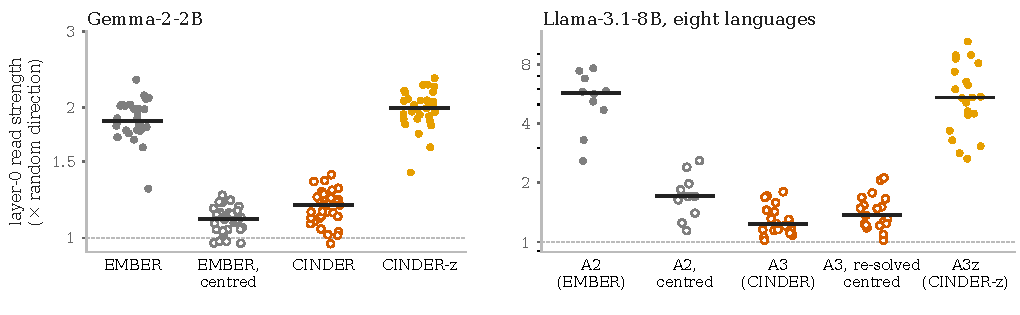
\includegraphics[width=\textwidth]{figures/read_decomposition.pdf}
  \caption{First-layer read strength of each edit relative to a random direction, per concept (dots) with medians (bars), on Gemma-2-2B (left) and the multilingual Llama-3.1-8B fits (right). Centring \ember{}'s dictionary brings its read strength down to \cinder{}'s on Gemma and most of the way on Llama; adding the mean term back (\cinderz{}, A3z) raises it again. Filled: uncentred edits; open: centred.}
  \label{fig:read}
\end{figure*}

\paragraph{The dictionary step does not depend on the metric}
Write $A_c = A - \mu_B\mathbf 1^{\top}$ for the centred embeddings.
The sharpened fit alternates $\tilde Z \leftarrow \tilde X Y^{\top}(YY^{\top}+\lambda I)^{-1}$ on $\tilde X = TA_c$ with a masked coefficient update, and \cinder{} maps the dictionary back as $T^{-1}\tilde Z$.

\begin{proposition}
\label{prop:metric}
For invertible $T$, $B \in \R^{d\times n}$, $Y \in \R^{k\times n}$ and $\lambda \ge 0$ with $YY^{\top} + \lambda I \succ 0$,
\begin{align*}
  &\arg\min_Z \|T(B - ZY)\|_F^2 + \lambda\|TZ\|_F^2 \\
  &\qquad = BY^{\top}(YY^{\top}+\lambda I)^{-1},
\end{align*}
independently of $T$.
\end{proposition}

\begin{proof}
$Z \mapsto \tilde Z = TZ$ is a bijection, and in $\tilde Z$ the objective $\|TB - \tilde ZY\|_F^2 + \lambda\|\tilde Z\|_F^2$ is strictly convex with minimizer $\tilde Z^* = TBY^{\top}(YY^{\top}+\lambda I)^{-1}$; hence $Z^* = T^{-1}\tilde Z^* = BY^{\top}(YY^{\top}+\lambda I)^{-1}$.
\end{proof}

\noindent At convergence of the fit, the mapped-back dictionary is therefore the Euclidean least-squares dictionary of the \emph{centred} embeddings, $Z_c = A_cY^{\top}(YY^{\top}+\lambda I)^{-1}$, for the affine model $\e_t \approx \mu_B + Z\mathbf y_t$ (on Gemma, $\|T^{-1}\tilde Z - Z_c\|/\|Z_c\| \le \expnum{0.008}$ in all \expnum{137} runs).
The coefficient step is where the metric matters: $Y$ is an $M$-orthogonal projection with $M = T^{\top}T$, so whitening chooses which tokens are grouped and how they are weighted.

\begin{proposition}
\label{cor:mean}
\cinderz{}'s dictionary (Eq.~\ref{eq:cinderz}) is $Z_z = Z_c + \mu_B\mathbf b^{\top}$ with $\mathbf b = (YY^{\top}+\lambda I)^{-1}Y\mathbf 1$, so its edit is $\cvec^{z}_t = \cvec_t + \beta_t\mu_B$ with $\beta_t = \sum_{i\in\Fc} b_i Y_{i,t}$.
\end{proposition}

\begin{proof}
Substitute $A = A_c + \mu_B\mathbf 1^{\top}$ in Eq.~\ref{eq:cinderz}.
\end{proof}

\noindent In the data, $\cvec^z_t - \cvec_t$ has at least \expnum{0.9995} of its energy along $\mu_B$ in every run (Gemma \expnum{137}, Llama \expnum{21}).
For a feature of width $w$ with same-sign coefficients of size about $1/\sqrt w$, $\beta_t \approx 1$ whatever $w$, so at $\delta = 1$ an uncentred edit subtracts roughly one full $\mu_B$ (observed median $\beta$: \ember{} \expnum{0.66}, \cinderz{} \expnum{0.56}, \cinder{} \expnum{0.05}; the edited tokens' own coordinate along $\mu_B$ is \expnum{1.06}).
The affine model also reconstructs raw embeddings better than the uncentred one (relative error \expnum{0.917} vs.\ \expnum{0.932}, 137 of 137 runs).

\paragraph{Where the read-strength gap comes from}
Concept means on Gemma-2-2B; $\perp\mu$: with $\hat\mu_B$ projected out of the edit.

\begin{center}
\footnotesize
\setlength{\tabcolsep}{2.5pt}
\begin{tabular}{@{}lcccc@{}}
\toprule
Edit & Read & $\hat\mu_B$ share & Read $\perp\mu$ & $\cos(\cvec_t,\e_t)$ \\
\midrule
\ember{} & \expnum{1.86} & \expnum{0.44} & \expnum{1.31} & \expnum{0.50} \\
\ember{}, centred $Z$ & \expnum{1.09} & \expnum{0.07} & \expnum{1.31} & \expnum{0.35} \\
\cinder{} & \expnum{1.18} & \expnum{0.05} & \expnum{1.32} & \expnum{0.30} \\
\cinderz{} & \expnum{1.99} & \expnum{0.48} & \expnum{1.32} & \expnum{0.50} \\
\bottomrule
\end{tabular}
\end{center}

\noindent \ember{} vs.\ \cinder{}: $+0.68$ read (27 of 27 concepts), but $-0.01$ once $\hat\mu_B$ is removed ($p = 0.44$), with the same Rayleigh ratio of the background covariance along the edit (\expnum{4.3} vs.\ \expnum{4.4}).
Across all edits, read strength follows the share along $\hat\mu_B$ (Spearman \expnum{0.75}) more closely than the background variance along the edit (\expnum{0.63}).
The mean term is also most of what aligns an uncentred edit with its token: with $\hat\mu_B$ removed from both, $\cos(\cvec_t, \e_t)$ is \expnum{0.31} for \ember{} and \expnum{0.29} for \cinder{} ($p = \expnum{0.15}$).
The read strength of the eigendirections of $\Sigma_B$ is U-shaped in their variance (top decile \expnum{1.08}, middle deciles \expnum{0.81--0.88}, bottom decile \expnum{1.59}, lowest 1\% \expnum{3.4}); strongly read directions concentrate on a few coordinates with a large first-layer normalization weight.
On Llama, A3z exceeds A3 by \expnum{$+4.48$} in read strength, of which \expnum{$+4.34$} is the mean term; $\hat\mu_B$ is read at \expnum{20.4$\times$}, so a \expnum{7\%} share suffices.
\paragraph{What the first layer does with the mean}
Setting the layer-0 normalization weight to one lowers $\hat\mu_B$'s read gain from \expnum{2.93$\times$} to \expnum{2.10$\times$} and the \ember{}--\cinder{} gap by \expnum{53\%}; zeroing its eight largest entries (\expnum{3.98--5.97}, against a median of \expnum{1.17}) lowers them to \expnum{1.74$\times$} and \expnum{75\%}; with $\hat\mu_B$ projected out, every edit is read at \expnum{1.28--1.35$\times$} under all three settings.
In the forward pass (50 tokens from 5 runs, each direction relative to random ones), the linear proxy predicts the measured layer-0 write well (Spearman \expnum{0.76--0.81}), and the mean and uncentred directions push far more change into the \emph{later} positions of the prompt (\expnum{2.1--4.3$\times$}, against \expnum{0.8--1.2$\times$} for the centred ones).
Yet at small perturbations the centred directions change the token's own next-token distribution more (KL \expnum{5.4$\times$} for \cinder{}, \expnum{3.9$\times$} for centred \ember{}, \expnum{1.6$\times$} for the mean direction); at $s = 1$ the directions are close.
The mean direction is thus ``read strongly'' in that it spreads into the context, not in that it changes what the model predicts at the token.

\subsection{The Mean Term on Its Own}
\label{app:mean}

\begin{figure*}[t]
  \centering
  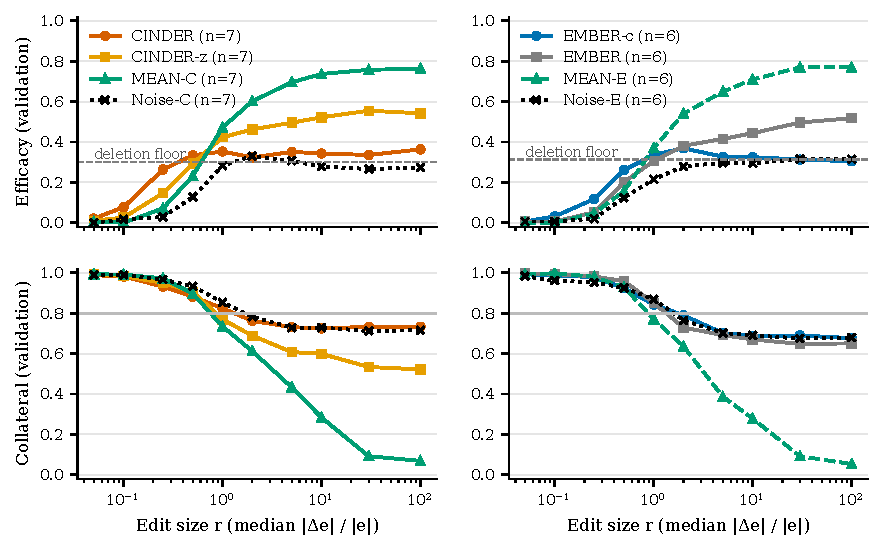
\includegraphics[width=0.85\textwidth]{figures/mean_curves.pdf}
  \caption{The mean term on its own (development runs, validation). Efficacy (top) and collateral (bottom) against edit size, mean over runs. Left: \cinder{}, \cinderz{}, the mean-only edit MEAN-C $= \beta^z_t\mu_B$ on \cinder{}'s tokens, and a random direction (7 runs). Right: \ember{}, \ember{} re-solved on centred embeddings (\ember{}-c), the mean-only edit MEAN-E on \ember{}'s tokens, and a random direction (6 runs). Dashed: deletion floor of the token set; grey: the collateral gate.}
  \label{fig:mean}
\end{figure*}

\paragraph{Design}
By Proposition~\ref{cor:mean}, \cinderz{}'s edit is \cinder{}'s plus $\beta_t\mu_B$, a term that carries no information about the concept.
We therefore evaluated that term alone (MEAN-C: $\e_t' = \e_t - \delta\beta^z_t\mu_B$ on \cinder{}'s tokens, with \cinderz{}'s own $\beta^z$), and the same split for \ember{} (\ember{}-c: \ember{}'s $Y$ and $\Fc$ with the dictionary re-solved on centred embeddings; MEAN-E: $\beta_t\mu_B$ with \ember{}'s coefficients), on the 8 development runs (Harry Potter, Ancient Rome and Valentine's Day; 7 with a \cinder{} edit, 6 with an \ember{} edit), over the same grid of $r$ and with the evaluation of App.~\ref{app:eval}.
The decompositions hold to a relative error of $10^{-4}$ in every run.
The test was pre-registered before any result (\path{results/paper_analysis/mean_edit/PREREG.md}); with three concepts, its statistics are descriptive.

\paragraph{The mean term erases by breaking the prompt}
Over $r \geq 1$, \cinderz{} removes \expnum{$+0.155$} more than \cinder{} (\expnum{7 of 7} runs), and the mean term alone removes more than \cinderz{} at every $r \geq 2$ (validation efficacy \expnum{0.60--0.76} vs.\ \expnum{0.46--0.55}) and more than a random direction of the same size (\expnum{$+0.48$} at $r \geq 10$, \expnum{7 of 7}; Figure~\ref{fig:mean}).
It does so by damaging the context: an unrelated multiple-choice question placed after a sentence with the edited word drops from \expnum{0.54} to \expnum{0.15--0.18} accuracy at $r \geq 10$, below chance, and collateral falls to \expnum{0.07}.
Across variants and sizes, efficacy above the deletion floor tracks this context damage (Spearman \expnum{0.54}, 63 points).
The centred edits destroy the words as completely at large $r$ (copy 0), yet stay near the floor with the context intact.
\ember{} shows the same pattern: centring its dictionary removes its large-$r$ gain (\expnum{$+0.097$} over $r \geq 1$, \expnum{6 of 6}) and its context damage, and raises efficacy at small edits (\expnum{$+0.07$} and \expnum{$+0.06$} at $r = 0.25$ and $0.5$).

\paragraph{Per unit of word damage, the centred edit erases most}
At the size where \expnum{90\%} of the edited words remain copyable, \cinder{} reaches efficacy \expnum{0.30}, \cinderz{} \expnum{0.20} and the mean term \expnum{0.13} (\ember{}-c \expnum{0.22}, \ember{} \expnum{0.15}, MEAN-E \expnum{0.11}); at \expnum{50\%} the three \cinder{} variants are equal.
Under the copy-gated rule, the mean term erases almost nothing (test efficacy \expnum{0.01}, against \expnum{0.12} for \cinder{} and \expnum{0.10} for \cinderz{}).
Under the collateral rule, however, it ties both (test $\Hthree$ \expnum{0.43} vs.\ \expnum{0.42} and \expnum{0.41}): collateral questions do not register damage to the rest of the prompt at $r \approx 0.5$.

\paragraph{Why the direction effect vanishes at $r = 1$}
The centred edits (\cinder{}, \ember{}-c, and \cinder{}'s direction on \ember{}'s tokens) reach a plateau near the deletion floor by $r \approx 0.5$--$1$, while \ember{} is still climbing, and keeps climbing past the plateau through generic damage.
On the 5 runs with all cells, centring \ember{}'s dictionary closes about a quarter of the gap to \cinder{}'s direction at $r = 0.5$ and nearly all of it at $r = 1$; the mean term becomes a net gain for \ember{} only at $r \geq 2$--$5$.

%=====================================================================
\section{Multilingual Erasure: Details}
\label{app:ml}
%=====================================================================

\paragraph{English erasure leaks}
In a first study we erased \ember{}'s 18 concepts from Gemma-2-2B-it with \ember{}, SNMF \citep{shafran2026constructing} and their combination, tuned every edit in English, and asked the held-out questions in English, German, Spanish, French and Russian.
Retention, the share of the concept knowledge left (1 = as before, 0 = chance), was on average \expnum{0.24} higher in the four other languages than in English under \ember{} (95\% CI \expnum{[0.15, 0.32]}), and \expnum{0.41} higher in Russian, where the English edit touches none of the concept's tokens.
SNMF, which edits MLP weights, erased all five languages about equally (\expnum{$+0.01$}), and adding \ember{} to it brought the gap back (\expnum{$+0.16$}).

\paragraph{Languages, model and data}
Llama-3.1-8B-Instruct in its eight supported languages: English, German, French, Italian, Portuguese, Hindi, Spanish and Thai.
The transformer runs in 4-bit NF4 and the edited embeddings in fp16, identically for every approach.
Concept sentences come from the concept's native Wikipedia page (via interlanguage links), up to 300 per language, topped up with NLLB translations of English sentences for short pages; neutral sentences come from native Wikipedia pages.
Shared fits use 30 concept and 30 neutral sentences per language.
The 20 held-out concepts are French Revolution, Tuberculosis, Cricket, Buddhism, Plutonium, Judaism, Karate, Existentialism, Prime number, The Matrix, Louvre, American Revolutionary War, Robot, Sigmund Freud, Giraffe, Surfing, Flush toilet, Cloud, Doctor of Philosophy and Tourism.
\ember{}'s English questions are used as published; German, French and Spanish come from existing translations; Italian, Portuguese, Hindi and Thai are machine-translated (NLLB and MADLAD candidates ranked by LaBSE, with script and number checks).
Questions for the new concepts were generated from the English page in \ember{}'s format, checked by a blind verifier and by automatic checks, and translated the same way.

\paragraph{Metrics and gates}
Per language $L$: efficacy (chance-corrected concept accuracy driven to chance), specificity (harmonic mean of Global-MMLU and similar-domain retention), fluency ($\min(1, \text{ppl}_{\text{orig}}/\text{ppl}_{\text{edit}})$ on 100 held-out native sentences), and $H_L$, their harmonic mean.
A concept's score is the mean $H_L$ over eligible languages (unedited accuracy $\geq 0.4$).
$\delta \in \{0.5, \dots, 200\}$ is chosen on validation, one value for all languages, and fails if MMLU or fluency drops below 0.9 of the unedited model in any language.
We report the \emph{strict} score (0 if a gate fails on test) and the \emph{ungated} one.

\paragraph{Approaches}

\begin{center}
\small
\setlength{\tabcolsep}{2.5pt}
\begin{tabular}{@{}lP{2.05cm}P{1.7cm}P{1.95cm}@{}}
\toprule
 & Fit & Selection & Edit \\
\midrule
A1 & 8 per-language \ember{} fits & TJ per language & each language's; overlaps resolved by page length \\
A2 & 1 fit on the 8-language sample, $Y$ extrapolated & TJ & \ember{}'s \\
A3 & A2 with \cs{} (8-language background) and \gs{} & \twj{} & mapped back \\
A3z & as A3 & as A3 & $Z$ re-solved on raw $E$ \\
\bottomrule
\end{tabular}
\end{center}

\paragraph{Results}
\expfill{Development table (18 concepts) and the pre-registered hypotheses H1--H3 on the 20 held-out concepts, with paired differences, CIs, win--loss counts and Wilcoxon $p$ (source: \texttt{results/ml/PREREG\_RESULTS.md}); the seed-coverage table; the seed-union follow-up (pooling selections over 3 fit seeds: \expnum{$+0.08$} for A3z, \expnum{19--4}, $p < 0.001$; pooled A1 and A3z tie at \expnum{0.30} vs.\ \expnum{0.31}).}

\paragraph{Why Hindi and Thai resist}
\ember{} edits only concept-only tokens, which never occur in the neutral sentences.
Llama splits Hindi and Thai words into short pieces that also occur in everyday text, so almost none qualify: on Baseball, \expnum{32\%} of English question tokens are concept-only, against \expnum{13\%} in German, \expnum{6\%} in Thai and \expnum{5\%} in Hindi, and the share of questions containing an edited token falls from \expnum{0.94} (English) to \expnum{0.00} (Hindi).
The same mechanism lets an edit made for one language act in every language that shares its pieces: Golf's per-language fit found its only feature in Thai, whose tokens cover \expnum{76\%} of the English questions.

\paragraph{Robustness}
Counts of concepts with an edit are stable across three fit seeds (A2: \expnum{9--12}; A3: \expnum{17--21} of 38), but which concepts are edited is not, and the edited token sets of one concept overlap by a Jaccard index of only \expnum{$\approx$0.2} across seeds, for every approach.
In \expnum{6} runs, across all approaches, a $\delta$ that passed both gates on validation failed one on test.

%=====================================================================
\section{Collateral-Aware Evaluation: Details}
\label{app:eval}
%=====================================================================

\subsection{Collateral Questions}
For every edited token with a common meaning outside the concept (e.g., \emph{Harry}, \emph{Caesar}, \emph{club}), LLM agents (Claude) wrote four-option multiple-choice questions that use the token in that meaning, and other agents reviewed them, both without knowing which methods would be scored.
Items that the unedited model answers incorrectly under either option order were dropped, and each split was frozen with a hash before any edited model was scored.
The held-out set has \expnum{3{,}501} items on \expnum{1{,}026} tokens.
Collateral accuracy is normalized against the unedited model per token, like \ember{}'s metrics.

\subsection{Scores, Gates and Selection Rules}
$\Hthree$ is the harmonic mean of efficacy, specificity and collateral; $H_4$ adds Alpaca coherence.
A point is admissible only if MMLU stays at or above 0.9 and validation collateral at or above 0.8 of the unedited model.
Each rule selects one grid point per run on validation and scores it once on test:

\begin{center}
\small
\setlength{\tabcolsep}{3pt}
\begin{tabular}{@{}lP{3.4cm}l@{}}
\toprule
Rule & Selects & Role \\
\midrule
Collateral & max $\Hthree$, both gates & primary \\
Paper & max $\hmean$(efficacy, specificity), MMLU gate & the old protocol \\
Fixed & the point $r = 0.5$ & equal edit size \\
Integrity & collateral rule, copy $\geq 0.9$ & words stay readable \\
\bottomrule
\end{tabular}
\end{center}

\subsection{Word Integrity Tests}
\begin{center}
\small
\setlength{\tabcolsep}{3pt}
\begin{tabular}{@{}lP{4.6cm}@{}}
\toprule
Test & Question asked \\
\midrule
Copy & Can the model repeat a sentence containing the word? \\
What is X? & Free answer, labelled blindly as knowing the concept (leak), knowing another meaning or not knowing (graceful), inventing a meaning (confabulation), or not registering the word (destruction) \\
Context & Is an unrelated MMLU question placed after a sentence with the word still answered? \\
Generation & Do 20 neutral prompts per concept that use the edited words keep their answer? \\
\bottomrule
\end{tabular}
\end{center}

\noindent Free-text answers were labelled by LLM agents that never saw which method produced them; 10\% of items were duplicated across agents, with agreement \expnum{0.92--0.97} on the exact label and \expnum{0.97--1.00} on the decisive class.
Each test is also run on the real word, the word deleted, and a nonce.
The \emph{nonce floor} and the \emph{deletion floor} are the efficacies of the unedited model on the concept questions with the edited words replaced by their nonces or deleted.

\subsection{Pre-registration and Robustness}
Analysis plans were written into a pre-registration and amendments, nearly all before their results existed (amendment 2, the intention-to-treat analysis and the McNemar test are exceptions).
The primary endpoint pairs only runs where both methods edit; Table~\ref{tab:robust} varies this and the collateral gate (all post hoc, defined after the primary result).

% Sources: results/varwidth/layers/collateral/confirm.md ("Primary" and "Sensitivity (amendment 9, post hoc)");
% Holm p of the gate rows: results/varwidth/layers/collateral/coverage_split.md ("both edit" columns).
\begin{table}[ht]
\centering
\footnotesize
\setlength{\tabcolsep}{2.5pt}
\begin{tabular}{@{}lcccc@{}}
\toprule
 & \multicolumn{4}{c}{$\Delta\Hthree$ vs.\ \ember{}} \\
\cmidrule(l){2-5}
Setting & \cinder{} & -RS & -z & -RS-z \\
\midrule
Primary & \expnum{$+.042$} & \expnum{$+.034$} & \expnum{$+.132$} & \expnum{$+.084$} \\
\quad Holm $p$ & \expnum{.41} & \expnum{.41} & \expnum{.074} & \expnum{.074} \\
All 60 runs & \expnum{$+.123$} & \expnum{$+.133$} & \expnum{$+.167$} & \expnum{$+.178$} \\
\quad Holm $p$ & \expnum{.10} & \expnum{.10} & \expnum{.10} & \expnum{.049} \\
Gate 0.9 & \expnum{$+.174$} & \expnum{$+.147$} & \expnum{$+.195$} & \expnum{$+.102$} \\
\quad Holm $p$ & \expnum{.012} & \expnum{.012} & \expnum{.008} & \expnum{.014} \\
Gate 0.7 & \expnum{$-.019$} & \expnum{$-.041$} & \expnum{$+.121$} & \expnum{$+.070$} \\
\quad Holm $p$ & \expnum{.73} & \expnum{.73} & \expnum{.27} & \expnum{.72} \\
Leave one out & \expnum{.03--.06} & \expnum{.01--.06} & \expnum{.11--.16} & \expnum{.06--.10} \\
\quad $p$ & \expnum{.08--.38} & \expnum{.16--.70} & \expnum{.004--.04} & \expnum{.004--.05} \\
\bottomrule
\end{tabular}
\caption{Robustness of the primary comparison (paired test $\Hthree$, unit = concept; 11 held-out concepts where both edit, 12 for all runs). Columns: \cinder{}, \cinder{}-RS, \cinderz{}, \cinder{}-RS-z. Primary: runs where both edit. All rows below it are post hoc. All 60 runs: a run without an edit is scored as the unedited model. Gate: the collateral rule rerun on the saved grids with the collateral gate at 0.9 or 0.7 instead of 0.8. Leave one out: range of the mean difference and of the uncorrected $p$ over the 11 omitted concepts.}
\label{tab:robust}
\end{table}

\paragraph{Development claims on held-out concepts}
The evaluation was developed on 3 concepts (Harry Potter, Ancient Rome, Valentine's Day; 8 concept-seeds) and then frozen.
Table~\ref{tab:devclaims} lists the development claims and what the 12 held-out concepts (60 runs) showed.
Of the eight claims, four replicate, one replicates only in part, and three do not; the development ordering of the variants, in particular, did not hold, so the main text compares methods only on held-out concepts.

% Sources: CINDER_collateral_evaluation.md, findings F1-F29 and F44 (development F1-F23, held out F24-F29, F44);
% numbers: results/varwidth/layers/collateral/{poc,confirm,twobytwo}.md.
\begin{table}[ht]
\centering
\footnotesize
\setlength{\tabcolsep}{3pt}
\begin{tabular}{@{}P{2.7cm}P{3.1cm}P{1.3cm}@{}}
\toprule
Development claim & Held-out result & Verdict \\
\midrule
Without collateral, selection picks destructive edits (\ember{} at $r = 10$--$100$ in \expnum{6 of 6} runs) & paper rule: \ember{} and \cinderz{} at median $r = \expnum{100}$; ours: every method at median $r = \expnum{1}$ & replicated \\
\addlinespace
At small $r$, \cinder{}'s direction removes more (efficacy \expnum{.33} vs.\ \expnum{.20} at $r = 0.5$, validation) & at $r = 0.5$, every variant beats \ember{} on \expnum{10 of 11} concepts (\cinder{} $\Delta\Hthree$ \expnum{$+.15$}, Holm $p$ \expnum{.012}) & replicated \\
\addlinespace
The gain is the direction, not the token set ($\Delta_{\text{dir}}$ efficacy \expnum{$+.15$} at $r = 0.25$, \expnum{$+.09$} at $r = 1$; 5 runs) & \expnum{$+.07$} at $r = 0.5$ (\expnum{10 of 11}, Holm $p$ \expnum{.097}); \expnum{$-.02$} at $r = 1$ & at $r = 0.5$ only \\
\addlinespace
At their own operating points the methods tie (test $\Hthree$ \expnum{.42} vs.\ \expnum{.42}) & \cinder{} \expnum{$+.04$}, Holm $p$ \expnum{.41} & replicated \\
\addlinespace
\cinder{}-RS is the strongest variant ($\Hthree$ \expnum{.46}) & \cinder{}-RS \expnum{$+.03$}; the -z variants lead (\expnum{$+.13$}, \expnum{$+.08$}) & not replicated \\
\addlinespace
The original-space edit (-z) does not help (\expnum{$-.01$} and \expnum{$-.06$} vs.\ its parent) & \cinderz{} \expnum{$+.13$} vs.\ \ember{} (\expnum{9 of 11}, Holm $p$ \expnum{.074}) & not replicated \\
\addlinespace
\cinder{} destroys fewer words (destruction \expnum{.21} vs.\ \expnum{.30}; exclusive words \expnum{.37} vs.\ \expnum{.74}) & \expnum{.52} vs.\ \expnum{.49}; exclusive \expnum{.70} vs.\ \expnum{.65} (n.s.) & not replicated \\
\addlinespace
Under the paper's rule \ember{} beats \cinder{}, and the -z edit reaches \ember{} by deleting the words & \cinder{} wins \expnum{1 of 11} concepts on $H_2$; \cinderz{} wins \expnum{11 of 11} at $r = \expnum{100}$ & replicated \\
\bottomrule
\end{tabular}
\caption{Development claims (3 concepts, 2--3 seeds) and their held-out test (12 concepts, 5 seeds, test split). Differences are paired against \ember{} on runs where both edit, unless stated otherwise.}
\label{tab:devclaims}
\end{table}

\paragraph{Mean and Noise (development only)}
Following \ember{}, Mean replaces each edited embedding by the vocabulary mean and Noise subtracts a random direction of the same length; both use the edited tokens of \ember{} or \cinder{} and the same grid, gates and selection (Table~\ref{tab:baselines}).
Mean has a single point ($r \approx \expnum{0.85}$--$\expnum{0.95}$), whose validation collateral is \expnum{0.71} (\expnum{0.55}--\expnum{0.78}), so it fails the collateral gate in every run and is never selected; at that point it deletes the words (3 labelled runs: copy \expnum{0}, destruction \expnum{0.99}) while the rest of the prompt is still read (context accuracy \expnum{0.52}--\expnum{0.54}).
Noise at its selected points (median $r = 1$; same 3 runs) destroys \expnum{0.25}--\expnum{0.35} of the edited words and still leaks the concept in \expnum{0.29} of the free answers.
We did not run the baselines on the held-out concepts.

% Source: results/varwidth/layers/collateral/poc.md ("Mean over concept-seeds"); Mean's point and the integrity numbers:
% CINDER_collateral_evaluation.md F7, F12, F15 (T3 labels on 3 runs).
\begin{table}[ht]
\centering
\footnotesize
\setlength{\tabcolsep}{3.5pt}
\begin{tabular}{@{}lccccc@{}}
\toprule
Method (tokens) & Runs & Eff. & Coll. & $\Hthree$ & mean $r$ \\
\midrule
\ember{} & \expnum{6} & \expnum{.22} & \expnum{.93} & \expnum{.42} & \expnum{0.76} \\
\quad Noise (\ember{}'s) & \expnum{6} & \expnum{.22} & \expnum{.91} & \expnum{.40} & \expnum{1.09} \\
\quad Mean (\ember{}'s) & \expnum{6} & \multicolumn{4}{c}{no admissible point} \\
\cinder{} & \expnum{7} & \expnum{.21} & \expnum{.87} & \expnum{.42} & \expnum{1.71} \\
\quad Noise (\cinder{}'s) & \expnum{7} & \expnum{.18} & \expnum{.89} & \expnum{.34} & \expnum{1.57} \\
\quad Mean (\cinder{}'s) & \expnum{7} & \multicolumn{4}{c}{no admissible point} \\
\bottomrule
\end{tabular}
\caption{Embedding-editing baselines on the development concepts (test split, collateral rule; mean over concept-seeds). A run without an admissible point is not edited.}
\label{tab:baselines}
\end{table}

\subsection{Integrity-Gated Selection}

\begin{figure}[t]
  \centering
  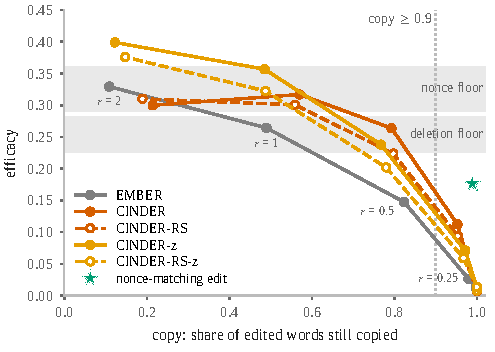
\includegraphics[width=\columnwidth]{figures/integrity.pdf}
  \caption{Removing more costs the words. Mean efficacy against the share of edited words the model can still copy, along the edit-size grid $r = 0.05, \dots, 2$ (labelled on \ember{}'s curve), over the held-out runs where each method edits (\expnum{41}--\expnum{55} of 60; validation questions). Grey bands: the efficacy of the unedited model when the edited words are replaced by their nonces (nonce floor, \expnum{0.29}--\expnum{0.36}) or deleted (deletion floor, \expnum{0.23}--\expnum{0.28}) in the test questions, over the five methods' token sets; dotted line: the integrity gate (copy $\geq 0.9$). Every method crosses its (test) deletion floor between $r = 0.5$ and $1$, where copy falls from about \expnum{0.8} to \expnum{0.5}, and none reaches its nonce floor while more than half of its words remain copyable. Star: the free nonce-matching edit on \cinder{}'s tokens (post hoc; seed 42, \expnum{9} runs, test split), which keeps \expnum{0.99} of the words copyable at efficacy \expnum{0.18}.}
  \label{fig:integrity}
\end{figure}
Figure~\ref{fig:integrity} shows the trade-off that this rule cuts through.
The integrity-gated rule (post hoc) is the collateral rule restricted to grid points where at least 90\% of the edited words can still be copied; the copy test was run at every grid point up to $r = 2$ (\expnum{1{,}530} points).
It coincides with the collateral-rule point in only \expnum{16} of \expnum{255} run-variants.
Table~\ref{tab:e3} gives the result.
On the paired endpoint of the primary analysis (runs where both edit), \cinder{} gains \expnum{$+0.096$} $\Hthree$ over \ember{} (95\% CI \expnum{$[-0.006, +0.214]$}, \expnum{7}--\expnum{3} concepts, Holm $p = \expnum{0.42}$) and \cinder{}-RS \expnum{$+0.092$} (\expnum{7}--\expnum{3}, \expnum{0.42}), the -z variants \expnum{$+0.029$} and \expnum{$+0.026$} (\expnum{0.75}).
Counting runs without an edit as no erasure, \cinder{} gains \expnum{$+0.134$} (\expnum{10}--\expnum{2}, Holm $p = \expnum{0.015}$) and \cinder{}-RS \expnum{$+0.166$} (\expnum{11}--\expnum{1}, \expnum{0.006}), the -z variants \expnum{$+0.053$} and \expnum{$+0.063$} (\expnum{0.33}).
The -z edits break copying at smaller $r$, so the rule pushes them to $r = 0.05$ in \expnum{24 of 52} and \expnum{26 of 55} runs.
Alpaca coherence at these points (seed 42) is \expnum{0.97--0.98} for every method.

% Source: results/varwidth/layers/collateral/last_mile.md ("E3: integrity-gated selection"); H4: last_mile.md Alpaca table,
% point e3 (seed 42); all-runs contrasts: coverage_split.md ("Integrity-gated"); r = 0.05 counts and 16/255:
% CINDER_collateral_evaluation.md F38.
\begin{table}[ht]
\centering
\footnotesize
\setlength{\tabcolsep}{2.4pt}
\begin{tabular}{@{}lccccccc@{}}
\toprule
Method & Runs & Eff. & Coll. & $\Hthree$ & $r$ & \shortstack{Copy\\ex./mu.} & $H_4$ \\
\midrule
\ember{} & \expnum{41} & \expnum{.06} & \expnum{.98} & \expnum{.12} & \expnum{0.1} & \expnum{.98/.99} & \expnum{.18} \\
\cinder{} & \expnum{52} & \expnum{.12} & \expnum{.97} & \expnum{.25} & \expnum{0.25} & \expnum{.96/.97} & \expnum{.35} \\
\cinder{}-RS & \expnum{55} & \expnum{.14} & \expnum{.98} & \expnum{.27} & \expnum{0.25} & \expnum{.94/.97} & \expnum{.20} \\
\cinderz{} & \expnum{52} & \expnum{.07} & \expnum{.99} & \expnum{.16} & \expnum{0.25} & \expnum{.97/.99} & \expnum{.16} \\
\cinder{}-RS-z & \expnum{55} & \expnum{.07} & \expnum{.99} & \expnum{.16} & \expnum{0.1} & \expnum{.98/.98} & \expnum{.25} \\
\bottomrule
\end{tabular}
\caption{Integrity-gated selection (copy $\geq 0.9$; post hoc) on the 12 held-out concepts, test split. Runs: runs with an edit (of 60); means over those runs; $r$: median edit size; copy for concept-exclusive and multi-meaning words separately; $H_4$ adds Alpaca coherence (seed 42 only, 8--10 runs).}
\label{tab:e3}
\end{table}

\subsection{Direction or Token Set}
\label{app:dir}

\begin{figure}[t]
  \centering
  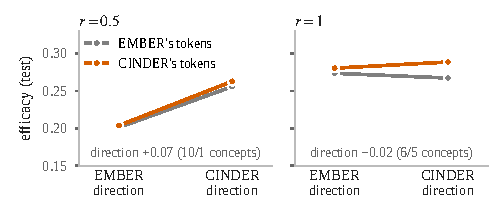
\includegraphics[width=\columnwidth]{figures/twobytwo.pdf}
  \caption{Test efficacy of the four direction $\times$ token-set cells (post hoc). At $r = 0.5$, switching to \cinder{}'s direction adds \expnum{$+0.07$} (\expnum{10 of 11} concepts) and switching to \cinder{}'s tokens \expnum{$+0.02$}, so the two lines nearly coincide; at $r = 1$ the direction effect vanishes (\expnum{$-0.02$}, \expnum{6}/\expnum{5} concepts). \ember{}'s own cell averages its 41 runs, the other cells 38.}
  \label{fig:twobytwo}
\end{figure}
Four cells cross the token set with the direction at a fixed $r = 0.5$, on the runs where \ember{} has a token set; ``\cinder{}'s tokens'' are \cinder{}'s top concept-only tokens, as many as \ember{} edits.
All cells use dense coefficients so that every token has a coefficient on $\Fc$.

\begin{center}
\small
\setlength{\tabcolsep}{4pt}
\begin{tabular}{@{}lcc@{}}
\toprule
Efficacy / $\Hthree$ & \ember{} direction & \cinder{} direction \\
\midrule
\ember{} tokens & \expnum{.20 / .39} & \expnum{.26 / .46} \\
\cinder{} tokens & \expnum{.20 / .39} & \expnum{.26 / .48} \\
\bottomrule
\end{tabular}
\end{center}

\noindent The direction effect (mean of the row differences) is \expnum{$+0.073$} efficacy and \expnum{$+0.097$} $\Hthree$, on \expnum{10 of 11} concepts (Holm $p$ \expnum{0.097} and \expnum{0.055}); the token-set effect is \expnum{$+0.016$} and \expnum{$+0.024$} (n.s.); the direction costs \expnum{0.02} collateral.
At $r = 1$ (secondary), the cell means are \expnum{.27 / .47} (\ember{} tokens, \ember{} direction), \expnum{.27 / .45} (\ember{} tokens, \cinder{} direction), \expnum{.28 / .46} (\cinder{} tokens, \ember{} direction) and \expnum{.29 / .48} (\cinder{} tokens, \cinder{} direction); the direction effect is \expnum{$-0.016$} efficacy ($p = \expnum{0.97}$) and \expnum{$-0.007$} $\Hthree$ ($p = \expnum{1.0}$), and the token-set effect \expnum{$+0.010$} and \expnum{$+0.012$} (both n.s.).

\subsection{The Nonce-Matching Edit}
\label{app:nonce}
We keep the model frozen and learn a change to each edited row.
The loss pushes the edited model, on concept sentences and new definitional prompts, toward what the unedited model does when the word is replaced by its nonce, while two further terms keep the word copyable (new carrier sentences) and keep the other meanings of multi-meaning tokens (sentences the model generated itself); no evaluation item is used for training.
The edit is either confined to the span of the edit set's concept components (rank $\leq 3$) or free, and is learned on \cinder{}'s or \ember{}'s token set; one free variant also adds concept questions that the model wrote itself to the forget data (+QA).
Selection is the integrity-gated rule; a run reaches the \emph{nonce point} when its test efficacy is at least its nonce floor minus 0.05, with copy $\geq 0.9$ and collateral $\geq 0.8$ (all post hoc, seed 42; Table~\ref{tab:nonce}).
The nonce floor averages \expnum{0.36} on the runs with \cinder{}'s tokens and \expnum{0.26}--\expnum{0.27} on those with \ember{}'s, and almost all runs that reach the nonce point have a floor near 0 (COVID-19 \expnum{0.00}, Pornography \expnum{0.07}--\expnum{0.11}); only Baseball (free, \ember{}'s tokens: \expnum{0.36} vs.\ floor \expnum{0.31}) and Heroin (+QA: \expnum{0.44} vs.\ \expnum{0.49}) reach a substantial floor.
Free edits move the rows far (median $r = \expnum{3}$, \expnum{3.2} and \expnum{1.6}) and keep them copyable, and remove \expnum{2--3$\times$} as much as integrity-gated \ember{} and \expnum{1.3--1.6$\times$} as much as integrity-gated \cinder{} on the same runs; paired $\Hthree$ against it (uncorrected): free (\cinder{}'s tokens) $-$ \cinderz{} \expnum{$+0.20$} (\expnum{7 of 9} concepts, $p = \expnum{0.055}$), +QA $-$ \cinderz{} \expnum{$+0.26$} (\expnum{7}--\expnum{1}, $p = \expnum{0.039}$), free (\ember{}'s tokens) $-$ \ember{} \expnum{$+0.28$} (\expnum{6}--\expnum{1}, $p = \expnum{0.047}$).
But asked ``What is X?'', the free edits repeat the word in only \expnum{0.34}--\expnum{0.49} of the answers (unedited word \expnum{0.96}, nonce \expnum{0.75}) and name a different invented string in \expnum{32}--\expnum{47\%} (nonce \expnum{17\%}), which the blind labels count as destruction.
Inside the concept subspace the words stay intact but almost nothing is removed, and the concept still leaks in \expnum{0.39} (\cinder{}) and \expnum{0.53} (\ember{}) of the answers.

% Source: results/varwidth/layers/collateral/nonce_edit.md (variants table; E3 baselines on the same runs; T3 labels;
% generation damage; renamed rate); attainment details: CINDER_collateral_evaluation.md F39-F43.
\begin{table}[ht]
\centering
\footnotesize
\setlength{\tabcolsep}{2.2pt}
\begin{tabular}{@{}lcccccc@{}}
\toprule
Edit (tokens) & \shortstack{Nonce\\point} & Eff. & Coll. & Copy & Destr. & Broken \\
\midrule
\multicolumn{7}{@{}l}{\emph{Learned, inside the concept subspace}} \\
\quad \cinder{}'s & \expnum{1/10} & \expnum{.04} & \expnum{.99} & \expnum{.99} & \expnum{.01} & \expnum{.02} \\
\quad \ember{}'s & \expnum{2/8} & \expnum{.02} & \expnum{.96} & \expnum{.97} & \expnum{.04} & \expnum{.04} \\
\multicolumn{7}{@{}l}{\emph{Learned, free}} \\
\quad \cinder{}'s & \expnum{2/9} & \expnum{.18} & \expnum{.86} & \expnum{.99} & \expnum{.50} & \expnum{.16} \\
\quad \ember{}'s & \expnum{3/7} & \expnum{.21} & \expnum{.86} & \expnum{.99} & \expnum{.59} & \expnum{.15} \\
\quad \cinder{}'s +QA & \expnum{3/10} & \expnum{.22} & \expnum{.89} & \expnum{1.00} & \expnum{.47} & \expnum{.15} \\
\midrule
\multicolumn{7}{@{}l}{\emph{Subtraction, integrity-gated (same runs)}} \\
\quad \ember{} & -- & \expnum{.07} & \expnum{.98} & -- & -- & -- \\
\quad \cinder{} & -- & \expnum{.14} & \expnum{.97} & -- & -- & -- \\
\quad \cinderz{} & -- & \expnum{.06} & \expnum{.99} & -- & -- & -- \\
\bottomrule
\end{tabular}
\caption{The nonce-matching edit (post hoc; seed 42, 12 held-out concepts, test split). Nonce point: runs that reach the nonce point, of the runs with an edit; Copy: share of edited words copied; Destr.: share of ``What is X?'' answers labelled as not registering the word; Broken: share of the 20 neutral prompts per concept whose answer breaks.}
\label{tab:nonce}
\end{table}

%=====================================================================
\section{Embedding-Space Analyses: Details}
\label{app:analyses}
%=====================================================================

All analyses in this section use the saved factorizations of 38 concepts $\times$ 5 seeds on Gemma-2-2B-it: \ember{}'s matrix with row sparsity (\ember{}), the sharpened matrix with row sparsity (\cs{}), and the sharpened matrix with global sparsity (\cs{}+\gs{}).
Unless stated otherwise, the concept feature of a run is identified without the judge, as the feature whose words match the concept's lexicon most often.

\subsection{Where the Concept's Energy Lies}
\label{app:energy}
\paragraph{Matrices and fits}
Raw $E_{\vs}^{\top}$; raw with $\hat\mu_B$ projected out; centred at $\mu_B$; whitened only ($\gamma = 0$); and \cs{}. Row-sparse fits, 38 concepts $\times$ 5 seeds; the 570 fits for the three intermediate matrices are new. A run ``finds'' the concept when its best feature has at least 5 lexicon words among its first 20 source words; no LLM judge is used.

\paragraph{Frequency}
Over 6.2M tokens of English Wikipedia, concept-only tokens are rarer than neutral-only ones in \expnum{35 of 38} concepts (median \expnum{9.4} vs.\ \expnum{12.9} per million), but their norms are not smaller (raw energy \expnum{0.9\%} larger). Across the vocabulary, a token's projection on $\hat\mu_B$ falls monotonically with its frequency (Spearman \expnum{$-0.69$} within a concept), and rare tokens put a smaller share of their centred energy on the top background directions (\expnum{0.07} vs.\ \expnum{0.65} at the frequent end). The tokens a raw concept feature collects are the rarest in $\vs$ (median \expnum{2.5} vs.\ \expnum{23} per million).

\paragraph{Seeded feature and full fits}
The seeded single feature (Figure~\ref{fig:mechanism}b) ends with purity \expnum{0.24} in the raw matrix, \expnum{0.04} centred and \expnum{0.27} with $\hat\mu_B$ projected out; whitening makes it pure (\expnum{0.86}, keeping \expnum{41\%} of the lexicon tokens) but ordinary (\expnum{70th} percentile of feature values), and sharpening raises its value to the \expnum{91st} percentile at the same purity (\expnum{37 of 38} concepts).
In full fits, a lexicon concept feature is found in \expnum{56\%} of raw runs, \expnum{61\%} with $\hat\mu_B$ projected out, \expnum{59\%} centred, \expnum{49\%} whitened only and \expnum{69\%} with \cs{}; per concept, raw $\to$ \cs{} is \expnum{15} better and \expnum{3} worse ($p = \expnum{0.011}$), and whitened only $\to$ \cs{} \expnum{17} and \expnum{0}.
The raw fit's best lexicon feature usually ranks near the top by $\rho$ (median rank \expnum{2}, against \expnum{1} under \cs{}; $p = \expnum{0.92}$); Harry Potter's raw rank is seed-dependent (\expnum{12, 1, 28, 48, 1}), while \cs{} ranks it first in all five seeds.

\paragraph{Selection-free directions}
The concept-minus-neutral mean direction, the top generalized eigenvector of concept vs.\ neutral second moments, and the top direction of the lexicon tokens do not rise in energy rank with \cs{} (e.g., lexicon direction rank \expnum{2} raw, which reflects $\hat\mu_B$; \expnum{9} without $\hat\mu_B$; \expnum{16.5} with \cs{}). What sharpening changes is the energy of the lexicon direction relative to whitening alone (\expnum{3.1$\times$} vs.\ \expnum{11.4$\times$} an average direction) and the value of the concept's cluster (App.~\ref{app:cs}).

\subsection{Feature Geometry and Norms}
\label{app:geometry}
\paragraph{Setup}
570 saved fits (\ember{}, \cs{} with row sparsity, \cinder{}), directions sign-aligned and compared in four metrics: the fit's own space, the raw embedding space (sharpened directions mapped back), the sharpened space (raw directions mapped forward), and the raw space with $\hat\mu_B$ projected out of every direction. Semantic relatedness of two features is the cosine of a small sentence encoder (all-MiniLM-L6-v2) between their source-word lists, independent of Gemma; token frequencies come from 32.6M tokens of Wikipedia.

\paragraph{Orthogonality}
Mean $|\cos|$ between directions:

\begin{center}
\footnotesize
\setlength{\tabcolsep}{3pt}
\begin{tabular}{@{}lccc@{}}
\toprule
Metric & \ember{} & \cs{}+RS & \cinder{} \\
\midrule
Own fit space & \expnum{.164} & \expnum{.052} & \expnum{.051} \\
Raw embedding space & \expnum{.164} & \expnum{.291} & \expnum{.258} \\
Raw, $\hat\mu_B$ projected out & \expnum{.079} & \expnum{.086} & \expnum{.079} \\
\bottomrule
\end{tabular}
\end{center}

\noindent Mapping sharpened directions back multiplies them by $T^{-1} \propto \Sigma_B^{1/2}$, which re-inflates the dominant background direction; $\hat\mu_B$ has cosine \expnum{0.82} with the top background principal component.

\paragraph{Neighbours and meaning}
The concept feature's nearest-neighbour angle is \expnum{50.6$^\circ$} (\ember{}), \expnum{73.6$^\circ$} (\cs{}) and \expnum{74.3$^\circ$} (\cinder{}); \ember{}'s neighbour is a recurring feature of rare names from the neutral sentences (\emph{Fulda}, \emph{Amiens}, \emph{Ferdinando}) at the \expnum{59th} relatedness percentile, the sharpened neighbours at the \expnum{92--94th}.
Over all pairs, the rank correlation of cosine with relatedness is higher for \ember{} (\expnum{0.33} vs.\ \expnum{0.24}), but \ember{}'s raw cosines largely track word frequency; controlling for it, \cs{} is higher (\expnum{0.34} vs.\ \expnum{0.25}), and among the top 0.5\% of pairs by cosine only the sharpened dictionaries are semantic (\expnum{75--79th} vs.\ \expnum{51st} percentile).
Mapped back to the raw space, sharpened cosines lose this property: it belongs to the metric in which they were found.
Projecting $\hat\mu_B$ out of \ember{}'s directions alone opens its nearest-neighbour angle from \expnum{50.6$^\circ$} to \expnum{74.0$^\circ$} (38 of 38 concepts), the sharpened level.

\paragraph{Norms}
The concept feature's norm is at the \expnum{82nd} percentile under \ember{} and the \expnum{57--61st} under \cs{}; \expnum{45\%} of its squared norm lies along $\hat\mu_B$ (typical feature \expnum{12\%}; \expnum{42\%} with the identification of App.~\ref{app:energy}), as does \expnum{97\%} of its excess squared norm over the run mean, and with $\hat\mu_B$ removed it falls to the \expnum{63rd}.
A token's coordinate along $\mu_B$ falls from \expnum{1.1} (rarest decile) to \expnum{0} (most frequent), so features built from rare tokens with same-sign coefficients collect about $\sqrt w\,\|\mu_B\|$ of norm. For Harry Potter, the raw feature is the 3rd to 6th largest of 100 by $\|\z_i\|$, with \expnum{0.67--0.80} of its squared norm along $\hat\mu_B$. Neither norm measures concept strength: with unit-norm coefficient rows, $\|\z_i\|$ is the scale of the support's vectors in the fit's metric.

\paragraph{Splits}
Two or more lexicon-matching features occur in \expnum{4--12\%} of runs (\expnum{15--28\%} by the judge). Blind labels of the 56 split pairs give \expnum{52} distinct sub-topics, \expnum{2} cuts of one concept and \expnum{2} off-topic pairs (e.g., batting vs.\ pitching, card games vs.\ betting). Ancient Rome has a Rome feature and an empire feature in all 15 runs; under \gs{} the Rome feature grows to \expnum{92--109} tokens and absorbs Roman persons, whereas \ember{}'s fixed 48 slots pad it with other capitals (Milan, Paris, Ottawa).

\subsection{Feature Widths and Tails}
\label{app:widths}
See App.~\ref{app:gs}.

\subsection{Abstract Concepts and Contamination}
\label{app:robustness}
\paragraph{Abstract concepts}
13 concepts that sit between broader topics (Romanticism, Utilitarianism, Baroque, Gothic architecture, Surrealism, Art Nouveau, Neoclassicism, Gnosticism, Existentialism at $|\Sc| = 300$; Stoicism, Epicureanism, Impressionism, Neoplatonism, whose pages are shorter, at $|\Sc| = 190$) and 4 entity controls (Harry Potter, Baseball, Uranium, Golf, at both sizes), 5 seeds, \ember{}, \cs{} and \cs{}+\gs{} (615 fits).
Each of the top 10 features by $\rho$ was shown, blind to condition, as its 20 strongest tokens with source words and labelled specific (P), broader (B) or unrelated (N) by two independent LLM annotators (agreement \expnum{0.94}, $\kappa = \expnum{0.88}$; parent topics fixed before any fit).
At $|\Sc| = 300$, a P feature is among the top 3 in \expnum{7\%} of abstract and \expnum{50\%} of entity runs under \ember{} (Mann--Whitney $p = \expnum{0.043}$), and \cs{} changes top-10 presence by \expnum{$+0.04$} (n.s.); \cs{}+\gs{} gains \expnum{$+0.22$} from two concepts (Baroque, Utilitarianism).
Stoicism illustrates the pattern: its top features are emotions, philosophy and religion, ethics and discourse words, and its most Stoic feature is a spelling feature that mixes \emph{Stoic} and \emph{stoa} with \emph{stock} and \emph{store}.

\paragraph{Contamination}
For Harry Potter, Baseball and Ancient Rome, a fraction $f \in \{0.1, 0.25, 0.5\}$ of the 300 concept sentences is replaced by sentences from adjacent pages (Harry Potter: Magic, The Lord of the Rings, The Chronicles of Narnia, Fantasy literature; Baseball: Softball, Cricket; Ancient Rome: Ancient Greece, Byzantine Empire), or, as a control added afterwards, from unrelated pages. Sentences naming the concept are dropped, and the sharpening target stays the concept's own page.
\ember{}'s mean rank of the best P feature rises from \expnum{4.1} to \expnum{6.9} at $f = 0.5$, equally with unrelated sentences (\expnum{5.9} vs.\ \expnum{5.7}, $p = \expnum{0.96}$), so the loss reflects fewer concept sentences rather than a fading contrast; for $f > 0$, \cs{} keeps it in the top 10 in \expnum{80--93\%} of runs, at a mean rank of \expnum{1.8--3.3}.
The share of the feature's top tokens that come only from the inserted sentences grows with $f$ (\ember{} \expnum{0.14 / 0.20 / 0.25}; \cs{} \expnum{0.05 / 0.13 / 0.14}); sharpening toward the contaminated sentences instead of the clean page raises it to \expnum{0.23} at $f = 0.5$. At $f = 0.25$, \ember{}'s Harry Potter feature mixes \emph{Tolkien}, \emph{Gandalf} and \emph{Hobbit} into the house and character names, whereas \cs{}'s at $f = 0.5$ keeps only Tolkien and Gandalf, at positions 16--20.

\subsection{Extrapolation Beyond the Sample}
\label{app:extrapolation}
\paragraph{Benchmark}
17 concepts with at least 80 page sentences outside the 300 sampled ones and a concept feature for both \ember{} and \cinder{} in some seed; on average \expnum{734} new concept-only token types per concept, plus new neutral token types from a 1{,}000-page Wikipedia sample (balanced: as many new neutral as new concept-only tokens; natural: one neutral sentence per new page sentence).
Three saved dictionaries, kept fixed (\ember{}; \cs{} with row sparsity; \cinder{}), 5 seeds.
Ground truth: blind labels as concept-specific (S), adjacent (A) or unrelated (U) on \expnum{5{,}196} tokens, written by LLM agents that saw only the concept, the token, its source words and a short context; agreement on 300 double-labelled items \expnum{0.90} ($\kappa = \expnum{0.82}$).

\paragraph{Rules}
Scores: projection on the concept feature, cosine, the coefficient of the joint dense least-squares solve, and the code share $y_{ft}|y_{ft}|/\|\mathbf y_{\cdot t}\|^2$.
Admission: the fit's own sparsity rule over the extended set (1\%), the saved absolute width, an in-sample cut-off ($|y_{ft}|$ at least the weakest coefficient of the saved support), the token's dominant feature, and share $\ge 0.5$.

\paragraph{Results}
Top-10 precision among new concept-only tokens is \expnum{0.18--0.27} for every dictionary and score (random \expnum{0.065}); counting adjacent tokens it is \expnum{0.49--0.69}, and no score separates concept-specific from adjacent tokens (AUC \expnum{0.40--0.48}).
The 1\% re-solve admits \expnum{15--22} tokens per run at precision \expnum{0.22--0.25}, about 37\% of them unrelated; fixed width and cut-off give the same precision, but fixing the width pushes out \expnum{13--15\%} of the original support, and Harry Potter's width grows from 48 to 59 under the 1\% rule.
Routing a token's shared meaning to other features (dominant feature or code share) does not help.
On \ember{}'s raw dictionary, projection on the concept feature mostly ranks rarity (Spearman \expnum{0.70} with Wikipedia rarity, against \expnum{0.25} for the joint solve); in the sharpened space the concept feature is nearly orthogonal to the rest of the dictionary (largest $|\cos|$ \expnum{0.28--0.30} vs.\ \expnum{0.64}), and projection and joint solve agree.
Recall is low: on six fully labelled concepts, re-solving the sparse codes recovers \expnum{4\%} of the concept-specific unsampled tokens.
\cinder{}'s wider features admit more concept-specific tokens per run at equal precision (\expnum{6.1} vs.\ \expnum{3.9}), and the sharpened dictionaries rank lexicon words higher (AUC \expnum{0.91} vs.\ \expnum{0.67} with projection).
\expnum{87\%} of the unsampled page tokens occur once on the page (\expnum{52\%} of concept-only $\vs$ tokens), and precision rises with a token's page frequency, from \expnum{0.28--0.30} at one occurrence to \expnum{0.59--0.71} at ten or more (in-sample); at one occurrence, in-sample and extrapolated tokens are alike.
We recommend ranking by the joint solve, admitting with the in-sample cut-off, and preferring \cinder{}'s dictionary.
Figure~\ref{fig:extrapolation} shows both results.

% Source: results/paper_analysis/extrapolation/figures/fig_precision_at_k.json and fig_precision_vs_pagefreq.json
% (WP5 plot data), restyled by paper/figures/src/fig_extrapolation.py.
\begin{figure*}[t]
  \centering
  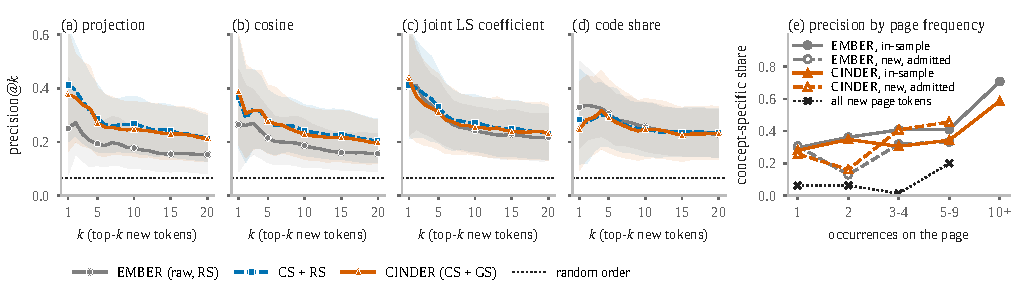
\includegraphics[width=\textwidth]{figures/extrapolation.pdf}
  \caption{Extrapolating a fixed dictionary to concept-only tokens outside the 300 sampled sentences (17 concepts, 5 seeds, balanced condition). (a)--(d)~Precision@$k$: share of the top-$k$ new concept-only tokens by each score that are blindly labelled concept-specific, mean over concepts with 95\% bootstrap bands; dotted: random order (\expnum{0.065}). (e)~Concept-specific share by the token's number of occurrences on the concept's page, for the tokens of the in-sample support (solid) and the new tokens admitted by the 1\% re-solve (dashed); dotted: all new page tokens. Bins with fewer than 5 concepts are omitted.}
  \label{fig:extrapolation}
\end{figure*}

%=====================================================================
\section{Qualitative Examples}
\label{app:examples}
%=====================================================================

\paragraph{The Harry Potter feature, before and after sharpening}
Table~\ref{tab:hp-tokens} lists the 48 tokens of the Harry Potter feature (1\% row sparsity, seed 42) on \ember{}'s raw matrix and on the sharpened matrix, by decreasing coefficient, written as the words they come from.
Both features open with 19 unmistakable Harry Potter tokens.
After that, the raw feature drifts into unrelated names, places and taxonomic suffixes, while the sharpened feature continues into the fictional world (Gringotts, Hogsmeade, Quidditch, McGonagall, Hagrid) and is more consistent across fragments of the same word (\textit{Gry}, \textit{Hog}, \textit{warts}).

\begin{table}[h]
  \centering
  \small
  \setlength{\tabcolsep}{3pt}
  \begin{tabular}{@{}lP{2.85cm}P{2.85cm}@{}}
    \toprule
    Ranks & \ember{} (raw) & \cinder{} (sharpened) \\
    \midrule
    1--19 & all Harry Potter (Gryffindor, Dumbledore, Slytherin, Rowling, Voldemort, Weasley, \dots) & all Harry Potter (Gryffindor, Slytherin, Dumbledore, Weasley, Hogwarts, \dots) \\
    \addlinespace
    20--30 & Kipling, \textbf{Ginny}, \textbf{Lupin}, Beatles, Arrondissement, Escondido, vice-chancellor, Cerambycidae, Alamos, Sherlock, Balompi\'e & \textbf{Hogwarts}, \textbf{Gryffindor}, \textbf{Ginny}, \textbf{Hogsmeade}, \textbf{Gringotts}, \textbf{Hogwarts}, \textbf{Lupin}, \textbf{Remus}, \textbf{Granger}, \textbf{Slytherin}, \textbf{JK} \\
    \addlinespace
    31--48 & \textbf{Remus}, Chrysomelidae, Trump, Nestl\'e, Bloomsbury, tesla, Fiennes, Polygyridae, Cerambycidae, Picasso, Assassins, Steelers, \textbf{Gryffindor}, Chhattisgarh, Lego, Kinect, Reagan, HBO & \textbf{Sirius}, \textbf{wand}, \textbf{McGonagall}, \textbf{Muggle}, \textbf{Ron}, \textbf{Goblet}, Sherlock, \textbf{Hagrid}, \textbf{Quidditch}, \textbf{Beauxbatons}, \textbf{potions}, \textbf{Rowling}, \textbf{Riddle}, \textbf{Grindelwald}, \textbf{Quirrell}, Holmes, \textbf{Merlin}, NHP \\
    \bottomrule
  \end{tabular}
  \caption{Tokens of the Harry Potter feature in \ember{}'s raw matrix and in the sharpened matrix (seed 42), shown as their source words. Bold: clearly Harry Potter tokens beyond rank 19. Ranks 20--30 hold 2 of 11 Harry Potter tokens before sharpening and 11 of 11 after.}
  \label{tab:hp-tokens}
\end{table}

\paragraph{Judge rejections}
\expfill{The descriptions and confidences of TJ's wrong rejections (Valentine's Day, Heroin, World War II; all at confidence 0.85), with the feature's top tokens.}

%=====================================================================
\section{Reproducibility and Cost}
\label{app:repro}
%=====================================================================

\paragraph{Code and results}
All code, pre-registrations and result files are in our repository.\note{Paths for the experiments pass; shorten for the final version.}
\begin{itemize}[leftmargin=*,itemsep=0pt,topsep=2pt]
\item Single-language fits and features: \path{experiments/varwidth/} (fitting \path{core.py}, data \path{prep.py}, selection \path{select.py}); sharpening \path{experiments/whitening/sharpen.py}.
\item Collateral-aware evaluation: \path{experiments/varwidth/erase_v2.py}, \path{collateral.py}, \path{integrity.py}, \path{last_mile.py}, \path{nonce_edit.py}, \path{confirm_stats.py}; pre-registration \path{results/varwidth/layers/PREREG.md}; results in \path{results/varwidth/layers/collateral/} (\path{confirm.md}, \path{last_mile.md}, \path{twobytwo.md}, \path{nonce_edit.md}).
\item Feature-level ladder and judges: \path{results/varwidth/layers/SUMMARY.md}, \path{experiments/varwidth/j3_eval.py}.
\item Multilingual study (branch \path{orip-ml}): \path{experiments/ml/}, \path{results/ml/PREREG_RESULTS.md}, \path{results/ml/UNION_RESULTS.md}.
\item Embedding-space analyses: \path{experiments/paper_analysis/}, \path{results/paper_analysis/}.
\item Figures: \path{paper/figures/src/}.
\end{itemize}

\paragraph{Compute and cost}
\expfill{GPU types and hours (NVIDIA TITAN Xp, RTX 2080 Ti and others on the university cluster); Gemini spend for feature judging, lexicons and question generation (about \expnum{16} NIS for the single-language ladder and about \expnum{17} NIS for the multilingual study).}


\end{document}
